
\chapter{对称性的恢复\label{chap:=005BF9=0079F0=006027=007684=006062=00590D}}

\section{引言}

在研究核相互作用的性质时（第4章），我们表明精确的多体Hamilton量 $H$ 在一些对称操作下是不变的，也就是说，它与相应的对称算符
$S$ 对易：
\[
[H,S]=0\tag{11.1}
\]

因此，我们总能找到同时是 $H$ 和 $S$ 本征函数的波函数。例如，线性动量 $\boldsymbol{P}$ 的三个分量、粒子数
$N$ 以及角动量算符 $\boldsymbol{J}^{2},J_{z}$ 。

我们还看到，这种一般性质在少数粒子的情况下非常有用，通过在对称算符的适当本征空间中工作，可以显著减小相应本征值问题的规模。两体系统中质心坐标的消除或应用于闭壳外少数粒子的角动量耦合技术就是例子。

在多粒子和强关联的一般情况下，对称性的恰当处理是一个严重的问题：一方面，我们想用简单的波函数来描述系统，比如独立运动粒子（或准粒子）的直积态；另一方面，如果我们同时要求恰当的对称行为，这样简单的波函数就无法考虑核子之间的重要关联。例如，唯一的平移不变直积波函数是平面波的乘积。它们肯定无法描述核子之间的强关联，正是这种关联导致它们聚集成一个有限的原子核。

然而在第2章中我们看到，这种关联可以用平均场（壳模型）来描述，并且壳模型波函数的直积态对许多核性质提供了非常合理的描述。然而，这样的波函数破坏了平移对称性。

这是一个普遍的过程\footnote{关于这一点的更详细讨论，见\cite{Li60a}}，在核物理中非常重要，即通过违反对称性的平均场方法来处理关联。这样的描述是否可行以及是否是一个好的近似当然取决于关联的性质。导致稳定形变的长程粒子-空穴关联以及提供超流性质的粒子-粒子关联，在任何情况下都是平均场类型的。在第7章中我们看到，它们可以用HFB理论来处理，这是一种违反角动量和粒子数守恒的平均场方法。结果表明，关联越强，这种近似就越好。类似于固体物理，我们说系统经历了向违反对称性状态的相变，例如向形变状态或超流相的相变。当然，当我们说原子核是局域化的、形变的或具有超流相时，经典和宏观的考虑进入了我们的论证。在本章后面我们将看到，相变的平均场描述在非常大（宏观）的系统中最终会变得精确。这意味着对于某些可测量的量，我们是在违反对称性的平均场方法中计算它们还是在不违反对称性的理论中计算它们可能无关紧要，当然，从量子力学原理上讲，后者是必需的。想象一个具有各种粒子数的量子流体$^{3}\mathrm{He}$的液滴。一旦液滴大到实际上可以“看到”，将液滴（或其平均场）视为局域化的（波包）肯定是一种精确的描述，尽管量子力学对于定态仍然需要平移不变的处理。

原子核当然不是宏观物体，但较重的原子核足够大，以至于对于宏观液滴最终会变得精确的平均场处理，对于某些量已经是非常好的描述。当然，这些量也是宏观定义的量，例如半径、形变\footnote{原子核的形变当然不像在宏观系统中那样是一个直接可测量的量，而只能以一种依赖模型的方式通过“内禀”四极矩相当间接地定义（见1.5节和附录B.2节）；一旦这种关系一劳永逸地建立起来，平均场理论在整个周期表中也能很好地再现原子核的形变。}、
超流电流、基态能量等。然而，那些具有量子性质的量，例如离散能谱和激发态之间的跃迁，将无法用纯平均场方法来描述。

特别地，直积波函数是对精确多体状态的一种非常糟糕的近似。正如我们将看到的，人们曾试图将违反对称性的波函数解释为在随原子核移动的“内禀”坐标系中的一个函数。所有仅依赖于这个内部函数的量最终在平均场方法中能得到很好的重现。

然而，有两个理由让我们寻找超越平均场的方法：
\begin{enumerate}
\item 在核物理学中，我们还对诸如跃迁概率和电磁矩等物理量感兴趣，而这些量绝不能仅从违反对称性的Nilsson波函数计算得出。
\item 原子核是一个有限系统。因此，相变总是会被抹平。我们经常会发现从守恒到弱破缺的逐渐转变，最终对称性会强烈破缺。在弱对称性破缺的情况下，我们必须超越平均场方法并恰当地纳入对称性。
\end{enumerate}
在11.2节中，我们首先希望更详细地讨论平均场方法中的对称性破缺机制。这将使我们更好地理解第5、6和7章中使用的方法。我们在此进行此讨论，是因为在那些章节中我们还没有第9和10章中的技术。

为了恢复在平均场方法中被破坏的对称性，人们尝试明确地转换到一个“内禀”系统。然而，这些尝试往往与基本困难紧密相连。另一方面，这些想法在许多唯象模型中被使用（见1.5节）。因此，我们将在11.3节中简要讨论它们。在从平均场方法获得的波函数基础上发展对称性守恒理论的常用方法是将波函数投影到对称算符的本征空间上。这些将在11.4节中讨论。

我们还将提到RPA近似。它超越了静态平均场方法，包含更高阶的关联，并提供对称性的近似恢复（见8.4.7节以及{[}UW 65, GW
68, MW 69b, MW 70, Bi 76, Ma 77a{]}）。正如我们将在12.3.2节中看到的，我们也可以在含时平均场理论中推导出这种方法，这表明这种更一般的平均场方法已经可以恢复对称性破缺的一些方面。

在本章中，我们主要探讨平移不变性（向局域化核的转变）、粒子数（向超流态的相变）和角动量（向形变态的相变）的对称性破缺。当然，还有其他对称性，如宇称\cite{BSB69}（在π介子凝聚的背景下{[}MKS
74, BF 74, BCD 75, BW 76{]}也会被打破）或同位旋（它只是一种近似对称性\cite{GW68}）。它们可以用非常相似的方式处理。

人们还研究了核物质具有由非平面波HF态描述的周期性长程有序晶体结构的可能性，这种结构违反平移对称性（Overhauser态{[}Ov
60, ALP 77, AAZ 77{]}）。人们发现，对于实际的核力，这样的波函数通常比平面波具有更高的能量。只有在非常低的亚核密度下，
$\alpha$粒子的稳定晶体结构才能形成（另见\cite{BC73}）。

本章讨论的对称性破缺是基于平均场方法的。当然，也有其他对称性破缺理论。它们有时可以用类似的技术来处理。

\section{平均场理论中的对称性破缺\label{sec:=005E73=005747=00573A=007406=008BBA=004E2D=007684=005BF9=0079F0=006027=007834=007F3A}}

正如我们在4.3节和第7章中所看到的，在原子核中存在非常不同的关联：一方面，存在非常短程的Brueckner关联，它与对称性破缺无关。另一方面，存在由ph和pp力引起的长程关联\footnote{然而，我们必须强调，这并不意味着产生这些关联的力的范围很大。}。
如果它们较弱，可以用RPA近似处理，并产生谐波集体振动和相关的基态。如果它们变得更强，我们会发现非谐性和能量大幅降低的模式（软模式）。相应的能量面在一个方向上变得非常平坦，并且在足够强的关联下，会出现突然的对称性破缺最小值。在这种情况下，\ref{chap:=0063A8=005E7F=007684=005355=007C92=005B50=006A21=00578B=00FF08HFB=007406=008BBA=00FF09}中讨论的平均场近似会产生非零的形变势
$\Gamma$ 或配对场 $\Delta$ 作为非线性“能隙方程”的解：

\[
\Gamma_{lm}=\sum_{rs}v^{\text{ph}}_{lsmr}\rho_{rs},\;\Delta_{lm}=\sum_{rs}v^{\text{pp}}_{lmrs}\kappa_{rs}\tag{11.2}
\]

其中$v^{\text{ph}}$和$v^{\text{pp}}$分别是ph和pp通道中的有效力，密度$\rho$和$\kappa${[}\ref{eq:=005355=007C92=005B50=005BC6=005EA6=0077E9=009635}{]}通过HFB方程\ref{eq:HFB equation}的对角化非线性地依赖于$\Gamma$和$\Delta$。

由于密度$\rho$和$\kappa$是用对称性破缺的波函数计算的，它们有一个单极部分$\rho_{0},\kappa_{0}$
、一个四极部分$\rho_{2},\kappa_{2}$等等。它们是通过将指标$r$和$s$耦合到角动量$I=0,2,\ldots$得到的，$\rho_{0}$对应于球形密度分布，并产生势$\Gamma$的球形部分$V_{0}$
。这在所有原子核中都很明显，对应于球形壳模型势。在下面我们将在此基础上进行研究。

取决于相互作用$v^{\text{ph}}$和$v^{\text{pp}}$的强度以及费米面附近的能级密度，“能隙方程”对于四极部分$\Gamma_{2}$
、单极配对场$\Delta_{0}$以及最终对于更高阶项也可能有非零解，这些在原子核中不太重要\footnote{例如，八极形变（$\Gamma_{3}$）或四极配对（$\Delta_{2}$）；另见4.4.7节中的多极展开。}。因此，我们可以将平均场分为三部分，
$V_{0}$ ，$\Gamma_{2}$和 $\Delta_{0}$ 。它们与平移对称性、转动对称性和粒子数的破坏有关。

在4.4.7节中我们看到，我们可以将相互作用 $v^{\text{ph}}$ 和 $v^{\text{pp}}$ 分解为具有不同角动量的分量。根据式（4.124）和（4.131），它们在角度上是可分离的。由于径向依赖性仅在核表面附近出现，我们可以用一个常数很好地近似它，对于$v^{\text{ph}}$的四极部分得到，并且从$v^{\text{pp}}$的单极部分得到著名的配对加四极模型（见7.4节）），我们将在下面关于原子核相变的讨论中使用它。

我们首先研究四极关联。在这种情况下，导致一体方程（11.2）的有效两体Hamilton量可以写成以下形式

\[
H=\sum_{k}\epsilon_{k}c^{\dagger}_{k}c_{k}-\frac{\chi}{2}\sum_{\mu}Q^{\dagger}_{\mu}Q_{\mu};\;\chi>0\tag{11.3}
\]

$c^{\dagger}_{k},c_{k}$ 是球形壳模型基中的粒子算符， $\epsilon_{k}$ 是 $T+V_{0}$
的相应本征值。四极算符$Q_{\mu}$由下式给出

\[
Q_{\mu}=\sum_{k_{1}k_{2}}\langle k_{1}|r^{2}Y_{2\mu}|k_{2}\rangle c^{\dagger}_{k_{1}}c_{k_{2}}\tag{11.4}
\]

“形变”方程（11.2）现在具有式（7.75）的形式，并确定形变参数 $q_{\mu}$ ：

\[
q_{\mu}=\chi\langle\Phi|Q_{\mu}|\Phi\rangle\tag{11.5}
\]

为了避免开壳层中HF的问题，我们进一步假设对于零相互作用 $\left(\chi=0\right)$ ，具有 $\epsilon_{i}\leq\epsilon_{F}$
的球形子壳层 $i$ 被占据，而具有 $\epsilon_{m}>\epsilon_{F}$ 的子壳层 $\epsilon_{m}$
是空的。

对于非零相互作用，系统的行为在很大程度上取决于费米面附近的平均能级间距\footnote{见6.3.5节中关于 $\Delta$ 的类似讨论。}
与强度 $\chi$ 的关系。例如，对于小的能级密度，对于幻核，或者对于 $\chi$ 的小值，我们有球形原子核的情况。“形变”方程（11.5）只有解
$q_{\mu}=0$ 。它对应于能量表面的一个最小值，我们可以在RPA框架{[}式（8.135）{]}中用频率 $\Omega$
计算振动状态：

\[
\frac{1}{\chi}=\sum_{mi}\left|\langle m\|r^{2}Y_{2}\|i\rangle\right|^{2}\frac{2(\epsilon_{m}-\epsilon_{i})}{(\epsilon_{m}-\epsilon_{i})^{2}-(\hbar\Omega)^{2}}\tag{11.6}
\]

随着能级密度的增加（即，如果我们研究远离封闭主壳层的原子核）或对于增加的强度 $\chi$ ，我们会达到一个点，此时RPA能量变为零，这等同于式（11.5）的球形解
${q}_{\mu}=0$ 不再对应于能量表面的最小值（见8.4.3节）。式（11.5）至少存在一个形变解 $\left|\Phi_{0}\right\rangle $
，其具有

\[
\langle\Phi_{0}|Q_{\mu}|\Phi_{0}\rangle\neq0\text{（至少对某个 }\mu\text{）}\tag{11.7}
\]

它违反了转动对称性。例如，我们现在能够通过函数$\left|{\Phi}_{0}\right\rangle $中质量分布的主轴来定义一个内禀坐标系。同时我们看到，现在有一整套HF方程的解$|\Phi\left(\Omega\right)\rangle$
，它们是通过由Euler角$\Omega=\left(\alpha,\beta,\gamma\right)$表征的空间任意转动从$\left|\Phi_{0}\right\rangle $得到的{[}见式（A.4）{]}

\[
\left|{\Phi\left(\Omega\right)}\right\rangle =\widehat{R}\left(\Omega\right)\left|{\Phi}_{0}\right\rangle \tag{11.8}
\]

如图11.1示意性所示。

\begin{figure}[H]
\begin{centering}
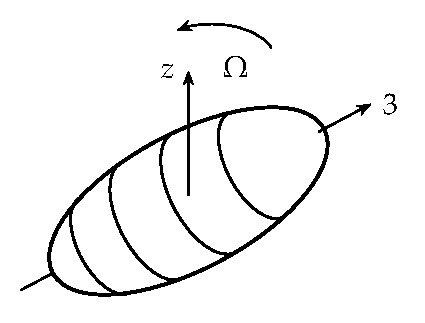
\includegraphics[width=0.48\linewidth]{pictures/11_1}
\par\end{centering}
\centering{}\caption{\label{fig:11_1}平均场方法定义一个内禀坐标系这一事实的示意表示。}
\end{figure}

由于Hamilton量的转动不变性，所有这些解具有相同的能量

\[
\langle\Phi\left(\Omega\right)\left|H\right|\Phi\left(\Omega\right)\rangle=\left\langle {{\Phi}_{0}\left|H\right|{\Phi}_{0}}\right\rangle .\tag{11.9}
\]

特别地，这意味着形变态不对应于最小值，而是对应于能量表面谷底的一个点。在11.4节中我们将看到，这种能量简并可用于构建所有这些波函数
$|\Phi\left(\Omega\right)\rangle$ 的线性叠加，它随后是对称算符 ${\boldsymbol{J}}^{2}$
和 ${J}_{z}$ 的本征函数。

从封闭主壳层附近的球形原子核到主壳层中间的形变原子核的转变通常称为相变。这类似于一个宏观系统，随着关联的增加我们有相同的机制：与对称性破缺相关的软模。然而，固态理论中的通常相变与核物理中的“相变”之间存在两个重要区别：

（i） 在宏观系统中，转变是严格不连续的，即不同的量（序参量）在连续参数的某个值处突然变化。对于有限系统，尖锐的转变被抹平，观察到由形变
${q}_{\mu}$ （或能隙 $\Delta$ ）给出的序参量有或多或少的逐渐变化。如果遵循我们的程序，这个事实有点隐藏起来：如果我们在RPA中围绕球形计算振动，我们发现随着耦合强度
$\chi$ 的增加，一个频率在尖锐的临界值 ${\chi}_{c}$ 处变为零。对于所有值 $\chi>{\chi}_{c}$
，我们找到一个形变解。然而，在有限系统中，两种方法——球形情况下的RPA和形变情况下的形变HF方法——在临界点附近失效，并且没有提供定量描述转变的方法。在一个精确解中，如图11.2示意性所示，我们发现在转变区域振动模的能量急剧降低，并在形变区域转变为
${2}^{+}$ 转动态，该转动态仅在非常大的形变或强关联的极限下变为零。

\begin{figure}[H]
\begin{centering}
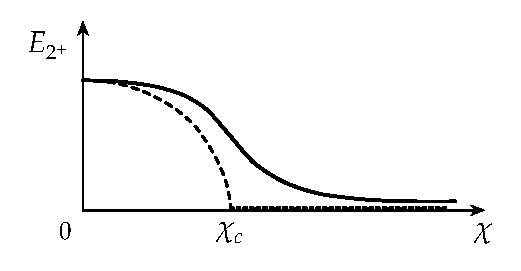
\includegraphics[width=0.5\linewidth]{pictures/11_2}
\par\end{centering}
\centering{}\caption{\label{fig:11_2}最低激发能作为四极耦合强度的函数的示意表示：精确解（实线）以及球形基中的RPA方法（虚线）和形变基中的RPA方法（点线）。在后一种情况下，最低的RPA解是赝态，它对应于转动（见8.4.7节）。}
\end{figure}

（ii） 在宏观情形下，平均场近似能够精确描述许多物理量，但在有限核系统中情况并非如此。正如我们将在11.4.4节中看到的，该近似仅在强对称性破缺的极限情况下才适用。在过渡区域存在许多原子核，静态平均场方法并不适用。从这个角度来看，线性动量、角动量和粒子数的三种对称性破缺非常不同。对于所有中等质量和重核，平均场近似在平移情形下的质量非常好。在转动情形下，它仅对形变良好的区域适用。然而，我们也观察到没有转动对称性破缺的球形核；也存在很大的过渡区域，平均场方法在那里失效。原子核中的BCS关联通常相当弱，因此相应的平均场近似，即BCS理论，往往不足以重现实验数据。因此，我们将在接下来的章节中研究改进平均场近似缺陷的方法。

四极关联强度的一种实验测量方法，因此也是平均场近似有效性的一种指示，由精确波函数 $|\Psi\rangle$ 中四极算符的涨落给出。

\[
\Delta{Q}^{2}=\langle\Psi\left|{Q\cdot Q}\right|\Psi\rangle-\langle\Psi\left|Q\right|\Psi\rangle\cdot\langle\Psi\left|Q\right|\Psi\rangle.\tag{11.10}
\]

（点表示五个四极算符的标量积。）由于在基态中期望值 $\left\langle {\Psi\left|{Q}_{\mu}\right|\Psi}\right\rangle $
在 $I=0$ 时为零，我们发现 $\Delta{Q}^{2}$ 与Hamilton量（11.3）的四极关联能成正比。

\[
\Delta{Q}^{2}=\langle\Psi\left|{\mathop{\sum}\limits_{\mu}Q^{\dagger}_{\mu}{Q}_{\mu}}\right|\Psi\rangle.\tag{11.11}
\]

四极力是吸引性的，因此系统希望在球形单粒子势 ${V}_{0}$ 中尽可能增加 $\Delta{Q}^{2}$ 。

另一方面，在实际原子核中存在关于 $\Delta{Q}^{2}$ 值的直接实验信息，因为它与非能量加权同位旋标量四极和规则成正比{[}见式（1.43）{]}。

\[
\Delta{Q}^{2}=\mathop{\sum}\limits_{\nu}{\left|\left\langle {\Psi}_{\nu}\parallel Q\parallel\Psi\right\rangle \right|}^{2}=5\cdot\mathop{\sum}\limits_{\nu}{BE2}\left({{2}^{+}_{\nu}\rightarrow0}\right).\tag{11.12}
\]

与能量加权和规则{[}式（8.159）{]}不同，能量加权和规则与 $\left\langle {r}^{2}\right\rangle $
成正比且大致为常数，非能量加权和在从球形到形变的转变过程中急剧增加：虽然巨四极共振的贡献大致保持不变，但最低 ${2}^{+}$
态的 ${BE2}$ 值从球形情形下的 $\sim{20}$ 单粒子单位{[}见式（B.85）{]}增加到形变情形下的 $\sim{100}$
，其中最低 ${2}^{+}$ 属于基态转动带。

四极强度在球形情形下集中在巨共振中，在形变情形下增加，然后集中在两个区域，即巨四极共振和集体转动。因此，在经典极限下，对于球形情形只有振动，而在形变情形下既有振动也有转动。

相变的进一步实验证据是“转动”谱的存在。在11.4节中我们将看到，在强对称性破缺的情况下，除了形变基态外，我们还得到一整个激发态带，它们与基态的区别仅在于对称算符
$S$ 的量子数。在那里，激发能与 ${S}^{2}$ 的本征值成正比。最简单的例子是形变核 $\left({\sim I\cdot\left({I+1}\right)/2\mathcal{G}}\right)$
中的转动带（$\sim I(I+1)/2\mathcal{J}$）、配对转动（$\sim(N-N_{0})^{2}/8\mathcal{I}_{N}$
\cite{Sch71a,BB76}）或平移激发（$\sim\boldsymbol{P}^{2}/2M$）。

相变也可以在玻色子图像中进行描述。一方面，我们在图9.5中看到，原则上我们可以通过费米子Hamilton量的玻色子展开来重现从球形到变形形状的转变。这些计算大多是在球形玻色子基中进行的。要在这个基中表示一个形变态需要非常复杂的波函数，因为我们总是在实验室坐标系中工作且不破坏转动对称性。另一方面，我们可以尝试用玻色子在内在坐标系中表示变形波函数：根据
Thouless 定理（E.26），我们可以用以下方式表示一个变形的Slater行列式。

\[
\left|{\Phi}_{0}\right\rangle =\mathcal{R}\exp\left({\mathop{\sum}\limits_{{mi}}{Z}_{mi}c^{\dagger}_{m}{c}_{i}}\right)|0\rangle,\tag{11.13}
\]

其中 $|0\rangle$ 是球形HF解， $\mathcal{R}$ 是归一化常数。在变形良好的情况下，我们有许多非零系数，即集体费米子对算符

\[
B^{\dagger}_{0}=\frac{1}{c}\mathop{\sum}\limits_{{mi}}{Z}_{mi}c^{\dagger}_{m}{c}_{i}\tag{11.14}
\]

其中

\[
{c}^{2}=\mathop{\sum}\limits_{{mi}}{\left|{Z}_{mi}\right|}^{2}
\]

在很好的近似下是一个玻色子（见9.2节），并且形变态

\[
|\Phi)=\mathcal{R}\exp(cB^{\dagger}_{0})|0)
\]

是一个仅包含集体玻色子 $B^{\dagger}_{0}$ 的相干态（见10.6.1节）。因此，我们将其称为玻色子 $B^{\dagger}_{0}$
的凝聚，类似于描述凝聚态物质某些类相变的玻色 - 爱因斯坦凝聚（另见\cite{SP77a}）。

对形变态的这种解释再次展示了平均场近似的经典行为。玻色子 $B^{\dagger}_{0}$ 的结构由变分方程（11.2）的解确定，一般来说它会随变形而变化。然而，我们可以证明，在小变形极限下，它恰好对应于RPA玻色子的
${ph}$ 部分，该部分在转变点处频率趋于零。从这个意义上说，我们可以说在相变过程中一个玻色子能量趋于零并形成凝聚。我们已经在BCS模型中使用了这个图像，在那里我们将BCS基态解释为Cooper对的凝聚。

到目前为止，我们的讨论主要集中在转动对称性的破坏上。接下来我们将表明，相同的考虑也可以应用于与配对关联相关的对称性破坏。这里我们首先研究简单的
辛弱数模型（见6.2节）。单个 $j$ 壳层中的有效Hamilton量由下式给出

\[
H=-G{S}_{+}{S}_{-}=-G\left({\boldsymbol{S}\cdot\boldsymbol{S}-{S}^{2}_{z}+{S}_{z}}\right),\tag{11.15}
\]

其中 ${S}_{i}$ 是在式（6.6）中定义的准自旋算符。它们作用于三维准自旋空间。 ${S}^{2}$ 和 ${S}_{z}$
与Hamilton量对易。因此，我们可以根据它们的辛弱数 $s$ {[}式（6.11）{]}和粒子数 $N$ 对本征态进行分类

\[
s=\Omega-{2S};\;\widehat{N}=2{S}_{z}+\Omega\tag{11.16}
\]

S由 $\Omega$ 个准自旋 ${\boldsymbol{s}}^{\left(m\right)}$ 组成{[}见图11.3和式（6.6）{]}。这个矢量的长度由辛弱数
$s$ 确定，并且我们将以下讨论限制在 $s$ 的一个固定值上。

\begin{figure}[H]
\begin{centering}
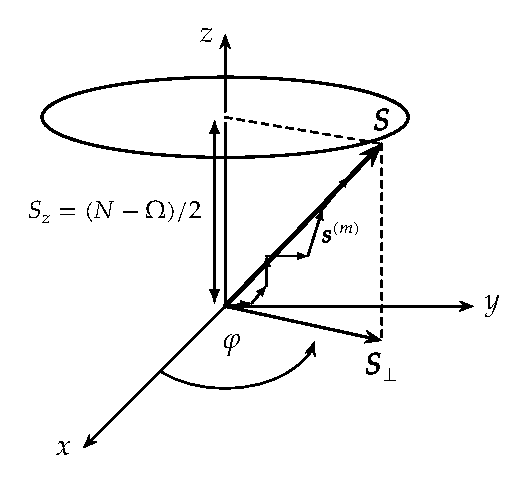
\includegraphics[width=0.46\linewidth]{pictures/11_3}
\par\end{centering}
\centering{}\caption{\label{fig:11_3}准自旋模型的示意图。}
\end{figure}

另一个量子数 ${S}_{z}$ 对应于绕 $z$ 轴的转动对称性。接下来我们将更详细地研究Hamilton量的这种不变性：

\[
\left\lbrack {H,\widehat{N}}\right\rbrack =0\text{ . }\tag{11.17}
\]

粒子数算符 $\widehat{N}$ 与 ${S}_{z}$ 相关（11.16），因此对应于准自旋空间中绕 $z$ 轴转动的无穷小生成元。这样的转动称为规范变换。相应的角度
$\varphi$ 是规范角。

我们可以用这个规范角表示算符 $\widehat{N}$

\[
\frac{\widehat{N}}{2}=-\frac{1}{i}\frac{\partial}{\partial\varphi}+\text{ const. }\tag{11.18}
\]

类似于用Euler角表示角动量算符 $\boldsymbol{J}$ ，如式（A.11）所示。

对于 $N$ 的固定值，即对于Hamilton量（11.15）的所有精确本征态 $|\Psi\rangle$ ，矢量S以频率

\[
\frac{d\varphi}{dt}=2\frac{dE}{dN}={2\lambda},\tag{11.19}
\]

绕对称轴进动，其中 $\lambda$ 是化学势{[}式（6.41）{]}。我们将这种运动称为配对转动。对于不同的粒子数，我们得到一个转动带（见图11.4）。

\begin{figure}[H]
\begin{centering}
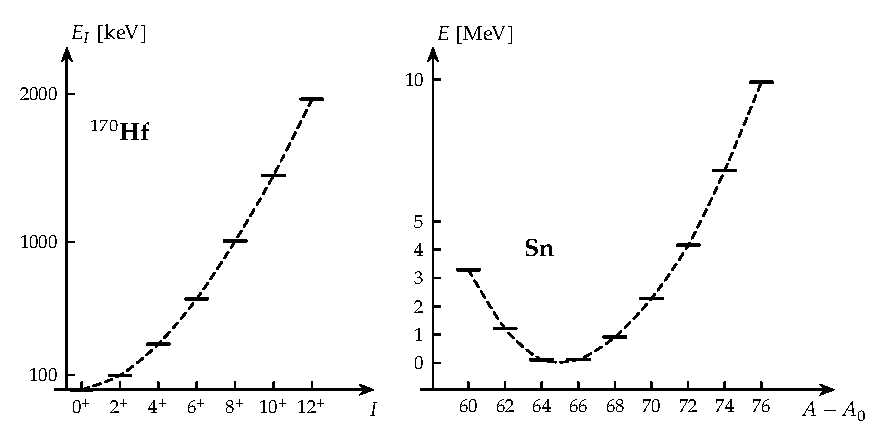
\includegraphics[width=0.62\linewidth]{pictures/11_4}
\par\end{centering}
\centering{}\caption{\label{fig:11_4}一个实验性的转动谱 $\left({^{170}\mathrm{{Hf}}}\right)$，其中激发能级对应于具有不同
$I$ 值的态，以及一个配对转动谱（Sn），其中“激发”能级对应于具有不同 $A$ 值的态（即相邻核中的基态）。（源自\cite{BB76}。）}
\end{figure}

${S}_{x}$ 和 ${S}_{y}$ 的期望值为零，

\[
\langle\Psi\left|{S}_{+}\right|\Psi\rangle=0,\tag{11.20}
\]

与上述讨论的情况中具有 $I=0$ 的精确基态的四极矩的方式相同。

$\boldsymbol{S}$ 在 $x,y$ 平面上投影的长度由下式给出

\[
{S}^{2}_{\bot}=\left\langle {\Psi\left|{{S}_{+}{S}_{-}}\right|\Psi}\right\rangle \tag{11.21}
\]

并且与关联能成正比。由于现在没有“球形”单粒子部分，系统在其基态总是倾向于 ${S}_{\bot}$ 的尽可能大的值，其中所有准自旋
${\boldsymbol{s}}^{\left(m\right)}$ 都是对齐的。因此，在这个模型中，对于所有力常数的值，我们都有一个“变形”态。对于大的
$S$ 值，即对于大的 $\Omega$ 值和 $N\ll\Omega$ ，我们因此可以预期通过打破规范对称性来获得精确波函数的良好近似。违反对称性的内态
$|\Phi\rangle$ 是一个BCS波函数。它由一个固定角度 $\varphi$ 表征。

\[
|\Phi(\varphi)\rangle=\mathop{\prod}\limits_{m>0}\left(u+ve^{\mathrm{i}\varphi}c^{\dagger}_{m}c^{\dagger}_{-m}\right)|-\rangle=e^{\mathrm{i}\varphi\widehat{N}/2}|\Phi(0)\rangle.\tag{11.22}
\]

通常的假设（6.31）对应于 $\varphi=0$ ，也就是说，我们以经典方式固定了角度。同样，所有态 $|\Phi\left(\varphi\right)\rangle$
在能量上是简并的。对称性破缺由能隙参数 $\Delta$ 来度量，它在转动情况下对应于变形方程（11.20）

\[
\Delta=G\left\langle {\Phi\left(0\right)\left|{S}_{+}\right|\Phi\left(0\right)}\right\rangle =G\mathop{\sum}\limits_{{m>0}}{uv}=G\cdot{\Omega uv}.\tag{11.23}
\]

系数 $u,v$ 由变分原理确定，这产生了通常的能隙方程{[}（6.60）和（6.65）{]}

\[
u=v=\frac{1}{\sqrt{2}}\tag{11.24}
\]

因此，BCS态也可以在准玻色子近似中由具有准玻色子 ${S}_{+}$ 的相干态来表示

\[
|\mathrm{BCS})=\mathcal{N}\exp(S_{+})|-)\text{ . }\tag{11.25}
\]

它违反了粒子数，但它具有适当粒子数 $N$ 的分量对应于系统的精确本征态（6.19）。对于大粒子数，相对涨落 ${\Delta N}/N$
（6.63）为零。因此，在这种情况下，平均场近似非常好。

在BCS理论更实际的应用中，除了单粒子部分外，我们还有纯配对力的模型

\[
H=\mathop{\sum}\limits_{k}{\epsilon}_{k}c^{\dagger}_{k}{c}_{k}-G\cdot P^{\dagger}P,\tag{11.26}
\]

\[
P^{\dagger}=\mathop{\sum}\limits_{{k>0}}c^{\dagger}_{k}c^{\dagger}_{k}
\]

现在不再可能有精确的解析解{[}KLM 61，RS 64，Ri 66{]}。它可以借助计算机求解，解表明BCS方法仍然是一个合理的近似，特别是如果我们只使用具有适当粒子数的分量（见第11.4节）。粒子数
$\widehat{N}$ 与Hamilton量对易；然而，相应的规范对称性被BCS近似打破，我们发现了一个相变。在所有细节上，该模型的工作方式与四极矩情况（11.3）完全类似。唯一的区别是我们现在必须对粒子数施加一个约束（通过在Hamilton量中添加一项
$-\lambda\widehat{N}$ ），因为我们对 $\widehat{N}$ 期望值为零的态不感兴趣。在转动对称性的情况下，我们有时也想要
${J}_{x}$ 期望值不为零的波函数。然后我们得到了转动模型（见第3.4节）。

为了展示从球形到变形的转变与从正常到超流系统的转变之间的紧密类比，我们给出以下相互对应的量的列表{[}Sch 71a，BHR 73{]}。

球形基中的模型Hamilton量是

\[
{H}_{Q}=\epsilon-\frac{\chi}{2}Q\cdot Q,\;{H}_{p}=\epsilon-GP^{\dagger}P.
\]

对于小耦合强度，基态是不相关联的球形壳模型态 $|0\rangle$ 。在RPA中考虑的剩余相互作用产生集体振动，即

四极振动 配对振动在

具有 $I=2$ 的核 质量为 $A\pm2$ 的核中。

它们增强了

BE2 值（在单对转移截面中

粒子单位）（以 ${2p}$ 单位）

${BE}\left({{2}^{+}\rightarrow{0}^{+}}\right)\simeq{20}{B}_{sp}\;\sigma\left({\text{ g.s. }\left({A-2}\right)\rightarrow\text{ g.s. }\left(A\right)}\right)\simeq{10}{\sigma}_{sp}.$

随着耦合强度增加，最低的RPA频率变为零。从这一点起存在一个

变形超流体

能量表面的最小值。它由基于球形（正常流体）基态 $|0\rangle$ 的直积波函数描述

\[
|\Phi\rangle=\mathop{\prod}\limits_{k}{\alpha}_{k}|0\rangle
\]

与准粒子算符

\[
\alpha^{\dagger}_{m}=\mathop{\sum}\limits_{k}{D}_{km}c^{\dagger}_{k},
\]

\[
\alpha^{\dagger}_{i}=\mathop{\sum}\limits_{k}{D}^{*}_{ki}{c}_{k},\;\alpha^{\dagger}_{i}={v}_{i}{c}_{i}+{u}_{i}c^{\dagger}_{i}.
\]

系数 ${D}_{kl}$ 和 ${u}_{k},{v}_{k}$ 由单粒子算符的对角化确定

\[
\epsilon-q\left({Q+Q^{\dagger}}\right),
\]

单粒子场的强度是序参量。它由“变形方程”和能隙方程自洽确定

\[
q=\chi\langle\Phi\left|Q\right|\Phi\rangle,\;\Delta=G\langle\Phi\left|P\right|\Phi\rangle.
\]

在准玻色子近似中，波函数 $|\Phi)$ 可写为相干态（玻色凝聚）

\[
|\Phi)\propto\exp(cB^{\dagger}_{0})|0),\quad|\Phi)\propto\exp(cA^{\dagger}_{0})|0),
\]

与玻色子

\[
B^{\dagger}_{0}=\frac{1}{c}\mathop{\sum}\limits_{{mi}}{Z}_{mi}c^{\dagger}_{m}{c}_{i},\;A^{\dagger}_{0}=\frac{1}{c}\mathop{\sum}\limits_{m}\frac{{v}_{m}}{{u}_{m}}c^{\dagger}_{m}c^{\dagger}_{m}+\frac{1}{c}\mathop{\sum}\limits_{i}\frac{{u}_{i}}{{v}_{i}}{c}_{i}{c}^{-}_{i}.
\]

平均场近似破坏了对称性。

\[
\left\lbrack {H,\widehat{J}}\right\rbrack =0,
\]

\[
\left\lbrack {H,\widehat{N}}\right\rbrack =0.
\]

其解 $|\Phi\rangle$ 表征了由坐标空间中的角度 $\Omega=\left({\alpha,\beta,\gamma}\right)$
以及准自旋空间中的角度 $\varphi$ 给出的一种取向。这些解对于转动是简并的

\[
R\left(\Omega\right)={e}^{{\mathrm{i}\alpha}{\widehat{J}}_{x}}{e}^{{\mathrm{i}\beta}{\widehat{J}}_{y}}{e}^{{\mathrm{i}\gamma}{\widehat{J}}_{z}},
\]

\[
G\left(\varphi\right)={e}^{{\mathrm{i}\varphi}\widehat{N}/2}.
\]

在形变状态下，我们在激发谱中有

$\beta,\gamma$ 振动 配对振动（含时形变）（含时能隙 $\Delta$ ）以及（作为无规位相近似法中的零频模式，见图11.4）

转动（具有 $I\neq0$ 的态） 配对转动（原子核中的基态）

\[
A\pm2,A\pm4,\ldots)\text{ . }
\]

基态“转动”带成员之间的跃迁与形变参数 $\left({q\text{ or }\Delta}\right)$ 的平方成正比。典型值为

\[
B\left({{E2},{2}^{+}\rightarrow{0}^{+}}\right)\simeq{100}{B}_{sp},\;\sigma\left({\text{ g.s. }\left({A-2}\right)\rightarrow\text{ g.s. }\left(A\right)}\right)\simeq{50}{\sigma}_{2p},
\]

\[
B\left({{E2},{2}^{\prime+}\rightarrow{0}^{+}}\right)\simeq3{B}_{sp},\;\sigma\left({\text{ g.s. }\left({A-2}\right)\rightarrow\text{ p. v. }\left(A\right)}\right)\simeq1{\sigma}_{2p}.
\]

转动可以（见11.4节）通过转动模型用经典方法处理：

\[
H-\omega{\widehat{J}}_{x},\;H-\lambda\widehat{N};
\]

或者通过投影用量子力学方法处理

\[
{P}^{I}_{MK}\propto\int{D}^{I*}_{MK}\left(\Omega\right)R\left(\Omega\right){\,\mathrm{d}\Omega},\;{P}^{N}\propto\int{e}^{-i\left({\varphi/2}\right)N}G\left(\varphi\right){d\varphi}.
\]

此列表总结了我们关于平均场理论中的对称性及其破缺的一般讨论，并且很明显，对于与对称性破缺相关的所有类型的相变，例如π介子凝聚，都可以列出类似的列表。我们现在将转向允许恢复破缺对称性的方法。

\section{向内禀系的变换\label{sec:=005411=005185=007980=007CFB=007684=0053D8=006362}}

\subsection{一般概念}

多体波函数中的对称性破缺与集体运动密切相关。为了更详细地解释这一事实，我们再次以转动对称性为例。一个形变波函数 $|\Phi\rangle$
在空间中定义了一个固定的取向，例如由质量分布的主轴来表征。所有仅在取向上与 $|\Phi\rangle$ 不同、但具有相同内禀结构并给出相同能量期望值的波函数
$|\Phi(\Omega)\rangle$ 都位于能量曲面的谷底。因此在经典图像中，我们有一种运动，如果它足够慢，就会靠近这个谷底。它对应于一种近似保持内禀结构的转动运动。如果形变很大，有许多粒子参与这种运动，我们就称其为集体运动。（关于这些准经典讨论的进一步内容，另见12.3节。）

在量子力学中，态 $|\Phi\left(\Omega\right)\rangle$ 跨越多体希尔伯特空间的一个子空间，即生成坐标方法（见第10章）意义下的集体子空间。如果这个子空间足够大——也就是说，正如我们将在11.4节中看到的，如果重叠
$\langle\Phi\left(\Omega\right)|\Phi\left({\Omega}^{\prime}\right)\rangle$
在 $\Omega={\Omega}^{\prime}$ 处强烈峰值化，这在强形变情况下会发生——它不仅大致包含基态，还包含具有相同内部结构且呈现转动谱的低激发态。

由于在这样一个波函数中的内禀结构在集体运动中大致保持，许多作者试图通过从 ${3A}$ 粒子坐标 ${\boldsymbol{r}}_{i}$
到集体坐标 ${q}_{1},\ldots,{q}_{f}$ 和内禀坐标 ${\xi}_{1}\ldots{\xi}_{{3A}-f}$
的适当坐标变换来分离内禀自由度和集体自由度{[}Vi 57a和b，Vi 58，SG 68，FKS 7{]}。

\[
\left({{\boldsymbol{r}}_{1},\ldots,{\boldsymbol{r}}_{A}}\right)\rightarrow\left({{q}_{1},\ldots,{q}_{f},{\xi}_{1},\ldots,{\xi}_{{3A}-f}}\right).\tag{11.27}
\]

集体坐标通常由基础对称性很好地定义为对称群生成元的正则共轭变量。在平移的情况下，有质心坐标；在转动的情况下，有一组角度作为Euler角；在超流体系中，它是规范角
$\varphi$ 。

内禀变量 $\xi$ 的定义是一个严重的问题。它仅在两个粒子的平移情况下很简单，此时它是相对坐标 $r={r}_{1}-{r}_{2}$
。在几个粒子的情况下，例如我们可以引入雅可比坐标，但在平移情况下的这个过程以及在转动情况下的类似过程在我们的多粒子系统中会变得极其复杂。然而，正如我们将在一些例子中看到的，我们有时可以在不明确指定内禀坐标的情况下推导出集体变量中的Hamilton量结构。

这些理论的主要思想是将核Hamilton量分解为以下三个部分

\[
H={H}_{\text{ coll }}\left(q\right)+{H}_{\text{ intr }}\left(\xi\right)+{H}_{\text{ coupl }}\left({q,\xi}\right),\tag{11.28}
\]

其中 ${H}_{\text{ coll }}$ 描述集体运动， ${H}_{\text{ intr }}$ 描述内禀运动。耦合项
${H}_{\text{ coupl }}$ ，希望它会很小或具有简单的结构。核平移的情况就是这个概念能很好发挥作用的一个例子。由于伽利略不变性，
${H}_{\text{ coupl }}$ 恒等于零。

如果我们可以忽略 ${H}_{\text{ coupl }}$ ，我们会发现总系统的本征函数是集体波函数 ${\chi}_{c}\left(q\right)$
和内禀波函数 ${\varphi}_{n}\left(\xi\right)$ 的乘积

\[
{\Psi}^{c}_{n}={\chi}_{c}\left(q\right)\cdot{\varphi}_{n}\left(\xi\right)\tag{11.29}
\]

并且能量具有以下形式

\[
{E}^{c}_{n}={E}_{c}+{E}_{n}.\tag{11.30}
\]

对于每个内禀态 ${\varphi}_{n}$ ，存在一个用指标 $c$ 标记的集体能带。

在这个过程的实际应用中，我们总是面临两个问题：

（i） 分解式（11.28）不是唯一的。它取决于内禀坐标的实际选择。显然，耦合项的大小敏感地依赖于这个选择。因此，有时会使用最小耦合变分原理来确定内禀系统{[}Co
56, BM 58, RV 69, Ru 73{]}。

（ii） 内禀Hamilton量 ${H}_{\text{ intr }}\left(\xi\right)$ 不依赖于 $A$
个粒子的 ${3A}$ 坐标，而仅依赖于 ${3A}-f$ 个变量 $\xi$ 。它们中没有一个能与粒子位置坐标等同。如果我们想在独立粒子图像中描述内禀运动，这就特别麻烦。在平移的情况下我们就已经有这个问题了。

因此，一系列作者使用了冗余变量的概念{[}LST 55, Li 55, Ta 56b, Na 57, Li 58, VC 70{]}。这里试图将正则变换方法的优点与处理
${3A}$ 个粒子坐标以描述内禀运动的优点结合起来。这是通过将 $A$ 体希尔伯特空间在粒子坐标 ${\boldsymbol{r}}_{1},\ldots,{\boldsymbol{r}}_{A}$
（物理子空间）中嵌入到一个维度为 ${3A}+f$ 的更大空间中来实现的，其中 $f$ 是集体变量的数量。我们用坐标 ${g}_{1},\ldots,{g}_{f}$
来表征这些额外的非物理自由度。然后物理子空间由以下条件表征

\[
{g}_{1}={g}_{2}=\cdots={g}_{f}=0.\tag{11.31}
\]

物理算符，即仅依赖于坐标 ${\boldsymbol{r}}_{1},\ldots,{\boldsymbol{r}}_{A}$ 的算符，例如Hamilton量，具有以下形式的本征函数

\[
{\Psi}_{mn}\left({g,\boldsymbol{r}}\right)={h}_{m}\left(g\right){\varphi}_{n}\left(\boldsymbol{r}\right),\tag{11.32}
\]

其中 ${h}_{m}\left(g\right)$ 是冗余坐标中的任意一组正交归一函数。因此，每个本征值 ${E}_{n}$
在扩大的空间中高度简并，但相应的本征函数在物理子空间（11.31）中是相同的\footnote{关于用冗余变量进行计算的更多细节，在量子力学情形下由 Lipkin 等人给出 \cite{LST55}，而对于经典理论由 Watanabe
给出 \cite{Wa56}。}。我们现在能够将冗余实验室系统中的坐标 ${g}_{1}\ldots{g}_{f},{\boldsymbol{r}}_{1}\ldots{\boldsymbol{r}}_{A}$
变换为具有集体坐标 ${q}_{1},\ldots,{q}_{f}$ 和粒子坐标 ${\boldsymbol{x}}_{1},\ldots,{\boldsymbol{x}}_{A}$
的冗余内禀系统中的坐标：

\[
{\boldsymbol{r}}_{i}={\boldsymbol{r}}_{i}\left({{q}_{1},\ldots,{q}_{f},{\boldsymbol{x}}_{1},\ldots,{\boldsymbol{x}}_{A}}\right),\;i=1,\ldots,A
\]

\[
{g}_{i}={g}_{i}\left({{q}_{1},\ldots,{q}_{f},{\boldsymbol{x}}_{1},\ldots,{\boldsymbol{x}}_{A}}\right),\;i=1,\ldots,f.\tag{11.33}
\]

通过这种方式，我们得到一个关于变量 $\boldsymbol{q}$ 和 $\boldsymbol{x}$ 的Hamilton量，其形式为

\[
H={H}_{\text{ coll }}\left(\boldsymbol{q}\right)+{H}_{\text{ intr }}\left(\boldsymbol{x}\right)+{H}_{\text{ coupl }}\left({\boldsymbol{q},\boldsymbol{x}}\right).\tag{11.34}
\]

在下一步中，我们对 ${H}_{\text{ intr }}$ 的对角化应用常规的近似技术。然而，问题仍然存在，即我们是否能找到一个合适的变换（11.33），使得耦合项很小，以及我们是否能以适当的方式分离通过这种近似得到的赝态的混合。在我们在平移和转动的背景下讨论这些技术之前，我们想提及类似的方法也已应用于更一般的集体运动，如表面振动，这些运动与对称性破缺无关{[}BP
53, Sü 54, MYT 55, To 55, MY 55, Co 55, MT 56, HM 57, Vi 57b{]}，但对于这些运动，人们也有兴趣推导集体Hamilton量。

\subsection{平移运动}

在下面我们将更详细地研究平移运动。这个简单的情形已经展示了许多问题。在核物理中，它与非常强的对称性破缺相关联。它是集体运动与内禀自由度完全解耦的唯一情形。其原因是伽利略不变性。

在这种情形下，内禀系统由质心参考系给出，集体坐标是

\[
\boldsymbol{R}=\frac{1}{A}\mathop{\sum}\limits_{i}{\boldsymbol{r}}_{i}\tag{11.35}
\]

在第一步中，我们不使用冗余坐标。在不指定内禀坐标 ${\xi}_{l}$ 的情况下，我们从（11.27）式得到导数

\[
\frac{\partial}{\partial{\boldsymbol{r}}_{i}}=\frac{1}{A}\frac{\partial}{\partial\boldsymbol{R}}+\mathop{\sum}\limits_{l}\frac{\partial{\xi}_{l}}{\partial{\boldsymbol{r}}_{i}}\frac{\partial}{\partial{\xi}_{l}}.\tag{11.36}
\]

由于内禀坐标 ${\xi}_{l}$ 仅依赖于差值 ${\boldsymbol{r}}_{i}-{\boldsymbol{r}}_{j}$
，我们得到 $\mathop{\sum}\limits_{i}\left({\partial/\partial{\boldsymbol{r}}_{i}}\right){\xi}_{l}=0$
并发现集体运动完全解耦

\[
H=-\frac{{\hbar}^{2}}{2m}\mathop{\sum}\limits_{i}{\left(\frac{\partial}{\partial{\boldsymbol{r}}_{i}}\right)}^{2}+V=\frac{1}{2Am}{\boldsymbol{P}}^{2}+\mathop{\sum}\limits_{{l{l}^{\prime}}}{D}_{l{l}^{\prime}}\left(\xi\right){\pi}_{l}{\pi}_{{l}^{\prime}}+V\left(\xi\right),\tag{11.37}
\]

质心动量为 $\boldsymbol{P}=\left({\hbar/i}\right)\partial/\partial\boldsymbol{R}$
，内禀动量为 ${\pi}_{l}=\left({\hbar/i}\right)\;\partial/\partial{\xi}_{l}$
，以及内禀惯性函数

\[
{D}_{l{l}^{\prime}}\left(\xi\right)=\mathop{\sum}\limits_{i}\frac{\partial{\xi}_{l}}{\partial{\boldsymbol{r}}_{i}}\cdot\frac{\partial{\xi}_{{l}^{\prime}}}{\partial{\boldsymbol{r}}_{i}}.\tag{11.38}
\]

如在上一节中所讨论的，我们不能用壳模型Hamilton量来近似（11.37）式的内禀部分。因此，我们现在应用冗余坐标方法。在这种情形下，坐标
${\boldsymbol{x}}_{i}$ 是质心参考系中的粒子坐标，对于变换（11.33）我们得到

\[
\boldsymbol{r}_{i}=\boldsymbol{x}_{i}+\boldsymbol{R},\quad\boldsymbol{x}_{i}=\boldsymbol{r}_{i}-\frac{1}{A}\sum_{j}\boldsymbol{r}_{j}+\boldsymbol{g},
\]

\[
\boldsymbol{g}=\frac{1}{A}\sum_{j}\boldsymbol{x}_{j},\quad\boldsymbol{R}=\frac{1}{A}\sum_{j}\boldsymbol{r}_{j}-\boldsymbol{g}.\tag{11.39}
\]

物理子空间由 $g=0$ 表征。对于动量，我们找到变换

\[
\frac{\hbar}{i}\frac{\partial}{\partial{\boldsymbol{r}}_{i}}=\frac{1}{A}\boldsymbol{P}+{\boldsymbol{p}}_{i}-\frac{1}{A}\mathop{\sum}\limits_{j}{\boldsymbol{p}}_{j},\tag{11.40}
\]

其中

\[
{\boldsymbol{p}}_{i}=\frac{\hbar}{i}\frac{\partial}{\partial{\boldsymbol{x}}_{i}},\;\boldsymbol{P}=\frac{\hbar}{i}\frac{\partial}{\partial\boldsymbol{R}}.
\]

在坐标 $\boldsymbol{x},\boldsymbol{R}$ 下的Hamilton量具有形式

\[
H=\frac{1}{2Am}{\boldsymbol{P}}^{2}+\mathop{\sum}\limits_{i}\frac{{\boldsymbol{p}}^{2}_{i}}{2m}+V\left({{\boldsymbol{x}}_{i}-{\boldsymbol{x}}_{j}}\right)-\frac{1}{2Am}{\left(\mathop{\sum}\limits_{i}{\boldsymbol{p}}_{i}\right)}^{2}.\tag{11.41}
\]

我们再次得到完全解耦。集体Hamilton量 $\left({1/{2Am}}\right){\boldsymbol{P}}^{2}$
具有平面波作为本征函数。对于每个内禀本征态，存在一个对应于平移运动的连续谱。由于我们只对内禀激发感兴趣，只研究 ${H}_{\text{ intr }}$
就足够了：

\[
{H}_{\text{ intr }}=\mathop{\sum}\limits_{i}\frac{{\boldsymbol{p}}^{2}_{i}}{2m}+V-\frac{1}{2Am}{\left(\mathop{\sum}\limits_{i}{\boldsymbol{p}}_{i}\right)}^{2}.\tag{11.42}
\]

它看起来与坐标 ${\boldsymbol{r}}_{i}$ 下的原始Hamilton量 $H$ 非常相似。只是有时被称为“反冲项”的
$\left({1/{2Am}}\right)\mathop{\sum}\limits_{{\mathrm{i}j}}{\boldsymbol{p}}_{i}{\boldsymbol{p}}_{j}$
项被减去了。我们现在能够用常规技术处理这个内禀Hamilton量。我们不必担心平移不变性，因为我们处于内禀系统中。例如，使用 Hartree-Fock
方法，我们会得到一个局域化的势和局域化的波函数。我们只需要考虑两件事：

（i） 我们必须从常规Hamilton量中减去包含两体相互作用的 $\left({1/{2Am}}\right)\mathop{\sum}\limits_{{\mathrm{i}j}}{\boldsymbol{p}}_{i}{\boldsymbol{p}}_{j}$
项。这在HF计算中经常做。在纯唯象壳模型中，我们有时至少从最终能量中减去这个算符的期望值。它是赝质心运动的动能。\footnote{如果我们在实验室系统（坐标 $\boldsymbol{r}_{i}$ ）中使用 Hamilton 量，并在 RPA 方法的框架内处理基态关联
{[}见式（8.111）{]}，会自动得到相同的项。它是与平移相关的零频率模对基态关联能的贡献。RPA 是一种对称性守恒理论，因此在这里没有必要引入冗余坐标。在其他对称性守恒理论中，如投影技术
{[}见第 11.4.4 节{]}，我们也会得到相同的项。}

（ii）我们必须意识到，由于我们使用了冗余坐标，在我们的本征函数中存在赝解。在我们精确求解质心框架下的问题的情况下，它们不会与物理解混合，并且可以通过特殊技术分离出来。然而，在近似解的情况下，它们可能会与物理解混合，有时很难确定哪些态是物理的，哪些不是。

为了更好地理解这些非物理解的结构，我们使用纯简谐相互作用\cite{GS57}

\[
V=\frac{k}{2}\mathop{\sum}\limits_{{i<j}}{\left({\boldsymbol{r}}_{i}-{\boldsymbol{r}}_{j}\right)}^{2}.\tag{11.43}
\]

在这种情况下我们可以写成

\[
{H}_{\text{ intr }}={H}_{0}+{H}_{1},\tag{11.44}
\]

其中

\[
{H}_{0}=\mathop{\sum}\limits_{i}\left({\frac{{\boldsymbol{p}}^{2}_{i}}{2m}+\frac{Ak}{2}{\boldsymbol{x}}^{2}_{i}}\right)\tag{11.45}
\]

以及

\[
{H}_{1}=-\frac{1}{2Am}{\left(\sum_{i}\boldsymbol{p}_{i}\right)}^{2}-\frac{A^{2}k}{2}{\left(\frac{1}{A}\sum_{i}\boldsymbol{x}_{i}\right)}^{2}.\tag{11.46}
\]

${H}_{0}$ 是一个单粒子简谐振子势，其本征函数为相应的Slater行列式。由于 ${H}_{1}$ 与 ${H}_{0}$
对易，它可以同时对角化，并且 ${H}_{\text{ intr }}$ 的精确解正是针对质心运动修正后的壳模型波函数。另一方面，
${H}_{1}$ 描述了在具有单个粒子频率 $\omega={\left(Ak/m\right)}^{1/2}$ 的简谐振子势中内禀坐标的质心
$\boldsymbol{g}=\left({1/A}\right)\mathop{\sum}\limits_{i}{\boldsymbol{x}}_{i}$
的一个振子。这种运动显然是虚假的（赝运动），因为在物理空间中我们有条件 $g=0$ 。赝解对应于壳模型势中原子核整体的振荡。

在基于简谐振子基的壳模型计算中，可以通过群论方法{[}BR 37, ES 55, UT 58, Kr 60, Ve 60, KM 66,
AMK 69, Mo 69, He 71, Sch 77b{]}将它们分离。由于质心问题在轻核中特别重要，并且另一方面，简谐振子势对于周期表中该区域的自洽场是一个合理的近似，所以这个基在许多实际应用中是首选的。

在一般情况下，问题非常复杂。通常很难精确分离赝分量。人们尝试通过在Hamilton量中添加一个算符 $S\left(g\right)$
来近似去除赝分量，该算符在物理空间 $\left({g=0}\right)$ 中为零，而在 $g\neq0$ 中很大且为正。它将赝本征态移到高能级，使得即使只是近似计算，它们也不会与低能态混合{[}Pa
67, SG 68, FKS 72{]}。

在重核中，在所有赝质心运动仅产生 $1/A$ 量级效应的情况下，可以忽略它。例如，我们计算一个在幻核构型之外有一个奇核子的原子核（例如，
${\mathrm{{Pb}}}^{209}$ 或 ${\mathrm{{Bi}}}^{209}$ ）的磁矩的轨道部分。第 $i$
个粒子相对于整个系统质心的轨道角动量由下式给出

\[
{\boldsymbol{l}}_{i}={\boldsymbol{x}}_{i}\times{\boldsymbol{p}}_{i}=\left({{\boldsymbol{x}}^{\prime}_{i}-\frac{1}{A}{\boldsymbol{x}}^{\prime}_{0}}\right)\times\left({{\boldsymbol{p}}^{\prime}_{i}-\frac{1}{A}{\boldsymbol{p}}^{\prime}_{0}}\right),\tag{11.47}
\]

其中 ${x}^{\prime}_{i},{p}^{\prime}_{i}$ 是幻核芯质心系统中粒子的坐标。下标0表征奇粒子。只有质子对磁矩的轨道部分有贡献。如果
$p$ 表征芯中的质子，我们得到

\[
\frac{\mu}{{\mu}_{k}}=\mathop{\sum}\limits_{p}{\mathrm{I}}_{p}+{g}_{l}\cdot{\mathrm{I}}_{0}
\]

\[
=\mathop{\sum}\limits_{p}{I}^{\prime}_{p}-\frac{1}{A}\left({\mathop{\sum}\limits_{p}{x}^{\prime}_{p}}\right)\times{p}^{\prime}_{0}-\frac{1}{A}{x}^{\prime}_{0}\times\left({\mathop{\sum}\limits_{p}{p}^{\prime}_{p}}\right)+\left({\frac{Z}{{A}^{2}}+{g}_{l}\left({1-\frac{2}{A}}\right)}\right){I}^{\prime}_{0}.\tag{11.48}
\]

根据奇粒子是质子还是中子， ${g}_{l}$ 分别为1或0。在一个中心与幻核芯质心重合的壳模型方法中，所有质子都处于闭壳层，式（11.48）中的前三项为零，我们得到一个针对质心运动
${\widetilde{g}}_{l}$ 修正后的 $g$ 因子：

\[
{\widetilde{g}}_{l}={g}_{l}\left({1-\frac{2}{A}}\right)+\frac{Z}{{A}^{2}}.\tag{11.49}
\]

这是一个 $1/A$ 效应。

\subsection{转动运动}

转动情形在形式上与平移情形有许多相似之处；然而，也存在一些基本差异：

（i） 在转动情形中不存在与伽利略不变性相对应的情况。因此，我们不能先验地期望集体运动和内禀运动之间解耦。我们只能希望耦合项至少对于不太大的角动量变得很小。它们有多大取决于内禀系统的选择。

（ii） 不存在明确界定的质心角。内禀系统最自然的选择似乎由质量分布的主轴提供。然而，结果表明系统围绕这些轴的赝运动会在内禀自由度和集体自由度之间产生非常大的耦合项
\cite{VC70}。

（iii） 基础对称群，即转动群，不再是阿贝尔群。虽然前两个困难在平面内的一维转动中就已经遇到了\footnote{BCS 波函数中规范对称性的破缺将对应于这样的一维转动。}，但我们在处理非对易算符时还有额外的困难。这需要一些涉及角动量代数的冗长计算，我们在此不想深入探讨。读者可参考相关文献获取所有细节
{[}LST 55, Na 57, Vi 57a, b{]}。我们仅给出主要结果。

作为集体坐标，选择了将实验室坐标系与体固定系统相连的Euler角 $\Omega=\left({\alpha,\beta,\gamma}\right)$
，其精确的定义仍未确定。在第一步中，我们再次可以尝试使用 $3\mathrm{\;A}-3$ 个内禀坐标 $\xi$ 。在这种情况下，Villars
{[}Vi 57a, b{]} 导出了Hamilton量的以下一般结构

\[
H=\frac{1}{2}\mathop{\sum}\limits^{3}_{{{\mathrm{i}k}=1}}{\left({\mathcal{I}}^{-1}\left(\xi\right)\right)}_{\mathrm{i}k}{\widehat{I}}_{i}\cdot{\widehat{I}}_{k}+\mathop{\sum}\limits^{3}_{{i=1}}{B}_{i}\left(\xi\right){\widehat{I}}_{i}+{H}_{\text{ intr }}\left(\xi\right).\tag{11.50}
\]

算符 ${\widehat{I}}_{i}$ 是角动量算符 $\boldsymbol{I}$ 相对于由Euler角表示的内禀轴
$i=\left({1,2,3}\right)$ 的分量 {[}见式 （A.14）{]}。Hamilton量的其余部分，特别是惯性张量
${\mathfrak{g}}_{\mathrm{i}k}$ 和量 ${B}_{i}$ ，仅取决于内禀坐标 $\xi$ 。它们提供了集体运动和内禀运动之间的耦合。

如果我们通过质量分布的主轴确定体固定系统，我们会发现张量 ${\mathfrak{g}}_{\mathrm{i}k}$ 是对角的，并且转动惯量由从无旋液滴运动导出的流体动力学值
（1.48） 给出。它们与实验证据有很大差异。因此，耦合项 ${B}_{i}$ 必须非常大。

我们也可以给出Hamilton量 （11.50） 的本征函数的一般结构。由于它是转动不变的，并且由于Wigner函数 ${D}^{1*}_{MK}\left(\Omega\right)$
在变量 $\Omega$ 中提供了一个完备系，我们得到式 （11.50） 的本征函数为：

\[
{\Psi}^{IM}\left({\Omega,\xi}\right)=\mathop{\sum}\limits_{K}{D}^{{I}^{*}}_{MK}\left(\Omega\right)\cdot{g}_{K}\left(\xi\right).\tag{11.51}
\]

与平移情形一样，坐标 $\xi$ 在实际应用中不是很有用。因此，几位作者使用了冗余坐标的概念。我们再次面临体固定坐标系的恰当选择问题。如果我们选择质量分布的主轴，我们又会得到流体转动惯量和大的耦合项。已经有几次尝试通过酉变换或内禀系统的恰当选择来消除它们
{[}Co 56, HM 57, BM 58, VC 70, Ru 73{]}。然而，一般来说，这样我们最终会得到非常复杂的方程。只有通过或多或少的严格近似才能求解它们。这类最详尽的研究是由Villars和Cooper
\cite{VC70} 进行的。他们得到了流体转动惯量的重整化，并最终得到了Thouless - Valatin值 {[}式 （8.113）{]}。

总结所有这些研究，我们可以说，向内禀系统的变换以及以此方式构建集体Hamilton量会遇到尚未完全解决的严重问题。只有在平移情形下，才能实现集体自由度和内禀自由度的完全分离，并且在简谐振子基的情况下，可以通过群论方法消除赝态效应。

然而，鉴于Bohr和Mottelson的转子模型取得了巨大成功（见第1章和第3章），我们应该预期，在转动情形下，至少也有可能实现集体运动和内禀运动的近似解耦。关键问题在于转动惯量的确定。与平动情形不同，在平动情形中总质量与剩余相互作用无关，而转动运动的惯性参数会受到关联的影响。这是一种动力学效应，很难通过纯粹的坐标变换来考虑。

处理对称性破缺的一种更为通用的方法是生成坐标法。在许多情况下，这些技术对应于向对称算符的相应本征空间的投影。我们将在下一节讨论这些投影方法。

\section{投影方法\label{sec:=006295=005F71=0065B9=006CD5}}

\subsection{投影算符}

投影技术是第10章中讨论的生成坐标法（GCM）的一种特殊情形。该方法的基本概念是在由一组依赖于一个或几个连续参数 $\Omega$
的生成函数 $|\Phi\left(\Omega\right)\rangle$ 所张成的子空间中，对完整的多体Hamilton量
$H$ 进行对角化。这个空间称为“集体子空间”。

我们现在有一个由与Hamilton量对易的对称算符 ${S}_{i}$ 生成的对称群，以及一个对称性破缺波函数\footnote{在下面的讨论中，我们始终考虑直积波函数，尽管该方法可以推广到其他类型的对称性破缺函数。}$|\Phi\rangle$。将该群的所有元素
$R(\Omega)$ 作用到 $|\Phi\rangle$ 上 ，我们得到一组连续的生成函数

\[
|\Phi(\Omega)\rangle=R(\Omega)|\Phi\rangle,\tag{11.52}
\]

其中 $\Omega$ 遍历群的整个参数空间。

所有波函数 $|\Phi\left(\Omega\right)\rangle$ 具有相同的能量期望值。因此，Peierls和Yoccoz\cite{PY57}提议在GCM技术中使用它们作为生成函数，即对系统的波函数
$|\Psi\rangle$ 提出以下拟设\footnote{关于基于 GCM 拟设的投影方法的综述，另见 \cite{Wo75}；关于更一般投影算符的综述，见 \cite{Ma70}。}：

\[
|\Psi\rangle=\int{\,\mathrm{d}\Omega f(\Omega)}|\Phi(\Omega)\rangle.\tag{11.53}
\]

能量相对于权重函数 $f\left(\Omega\right)$ 的变化对应于 $H$ 在由函数 $|\Phi\left(\Omega\right)\rangle$
所张成的空间中的对角化（见第10.2节）。这个子空间在对称群的元素作用下是不变的\cite{Ze67}：

\[
R\left(\Omega\right)|\Psi\rangle=\int d{\Omega}^{\prime}f\left({-\Omega+{\Omega}^{\prime}}\right)|\Phi(\Omega')\rangle,\tag{11.54}
\]
\footnote{请注意，对于非阿贝尔群，$-\Omega+\Omega'$ 取决于排序，并且表示与变换 $R^{-1}(\Omega)R(\Omega')$
对应的参数集。}

这意味着投影到这个子空间上的投影算符 ${P}_{\Phi}$ 与对称操作 $R\left(\Omega\right)$ 对易。因此我们看到，我们可以找到
${P}_{\Phi}H{P}_{\Phi}$ 和对称算符的同时本征函数。换句话说，存在一个使能量最小化并使 $|\Psi\rangle$
具有适当对称性的函数 $f\left(\Omega\right)$ 。

为了找到这样一个函数，我们在以变量 $\Omega$ 表示的对称算符的一组完备本征函数中展开 $f\left(\Omega\right)$
。对于所有阿贝尔群，这对应于Fourier分解。例如，我们考虑与粒子数破缺相关的规范群的情形（见第11.2节）。它有一个群参数 $\varphi$
，对称算符 $\widehat{N}/2$ 具有表示 $i\partial/\partial\varphi$ 。它的本征函数是指数函数

\[
f\left(\varphi\right)=\mathop{\sum}\limits_{n}\frac{1}{2\pi}{e}^{-{\mathrm{i}n\varphi}}\cdot{g}_{n}\tag{11.55}
\]

由于 $\varphi$ 中的周期性， $n$ 为整数。由式（11.53）和（11.55）我们得到

\[
|\Psi\rangle=\mathop{\sum}\limits_{n}{g}_{n}{\widehat{P}}^{2n}|\Phi\rangle,\tag{11.56}
\]

其中

\[
{\widehat{P}}^{A}=\frac{1}{2\pi}{\int}^{2\pi}_{0}{e}^{{\mathrm{i}\varphi}\left({\widehat{N}-A}\right)}{d\varphi}.\tag{11.57}
\]

算符 ${\widehat{P}}^{A}$ 在数学意义上是一个投影算符 $\left({{\widehat{P}}^{2}=\widehat{P},\widehat{P}^{\dagger}=\widehat{P}}\right)$
，它投影到具有粒子数的子空间上

A. 为了说明这一点，我们用单位算符从左和从右乘以 ${\widehat{P}}^{A}$ ，单位算符由具有粒子数 $N$ 的一组完备正交波函数
$|{N\alpha}\rangle$ 表示：

\[
{\widehat{P}}^{A}=\mathop{\sum}\limits_{{{N\alpha},{N}^{\prime}{\alpha}^{\prime}}}\left|{{N\alpha}\rangle\left\langle {{N\alpha}\left|{\frac{1}{2\pi}{\int}^{2\pi}_{0}{e}^{{\mathrm{i}\varphi}\left({\widehat{N}-A}\right)}}\right|{N}^{\prime}{\alpha}^{\prime}}\right\rangle \left\langle {{N}^{\prime}{\alpha}^{\prime}}\right.}\right|
\]

\[
=\mathop{\sum}\limits_{N\alpha,N^{\prime}\alpha^{\prime}}|N\alpha\rangle\langle N\alpha\mid N^{\prime}\alpha^{\prime}\rangle\langle N^{\prime}\alpha^{\prime}|\cdot\delta_{NA}=\mathop{\sum}\limits_{\alpha}|A\alpha\rangle\langle A\alpha|.\tag{11.58}
\]

由于我们只对具有适当粒子数 $A$ 的波函数 $|\Psi\rangle$ 感兴趣，我们得到

\[
{g}_{n}=0\text{ for }{2n}\neq A\text{ . }
\]

${g}_{A/2}$ 是一个归一化常数。

同样，在平移的情况下，我们得到一个投影算符，投影到具有本征值 $\boldsymbol{p}$ 的线性动量算符 $\boldsymbol{P}$
的本征态上：

\[
{\widehat{P}}^{\boldsymbol{p}}=\frac{1}{{\left(2\pi\hbar\right)}^{3}}{\int}^{+\infty}_{-\infty}{e}^{\left({\mathrm{i}/\hbar}\right)\boldsymbol{q}\left({\boldsymbol{P}-\boldsymbol{p}}\right)}{d}^{3}q=\delta\left({\boldsymbol{P}-\boldsymbol{p}}\right)\tag{11.59}
\]

以及

\[
{\widehat{P}}^{\boldsymbol{p}}\Phi\left({{\boldsymbol{r}}_{1},\ldots,{\boldsymbol{r}}_{A}}\right)=\int{d}^{3}q{e}^{i\boldsymbol{{pq}}/\hbar}\Phi\left({{\boldsymbol{r}}_{1}-\boldsymbol{q},\ldots,{\boldsymbol{r}}_{A}-\boldsymbol{q}}\right).
\]

因此，对于阿贝尔对称群，权重函数 $f$ 完全由纯运动学确定。

对于非阿贝尔群则不同。在这里，我们最终不会得到数学意义上的投影算符——尽管在这种情况下我们也使用“投影技术”这个术语。权重函数 $f$
并不完全由对称性确定。最重要的例子是三维转动的情况。由于这个对称群涉及许多细节，并且我们不想在这里打断投影技术的一般讨论，我们将在第11.4.6节中回到三维转动。

\subsection{变分前后的投影}

到目前为止，我们还没有指定违反对称性的内部波函数 $|\Phi\rangle$ 。原则上，有两种方法来确定这个函数

（i） 投影前变分 （VBP） \cite{PY57}。在这种情况下，例如，我们按照第7章中描述的方法进行，通过变分原理确定最优直积波函数
$|\Phi\rangle$

\[
\delta\frac{\langle\Phi\left|H\right|\Phi\rangle}{\langle\Phi\mid\Phi\rangle}=0;\tag{11.60}
\]

这个方程的一个“变形”解 $|\Phi\rangle$ 是相应对称算符本征态的叠加，例如角动量\footnote{由于在本节中我们仅对不同的投影技术进行非常定性的讨论，这里我们仅以角动量 $\hat{\boldsymbol{J}}$ 为例，而不深入转动群的细节。在以下内容中，$\hat{\boldsymbol{J}}$
可以被任何其他对称算符替代。} $\hat{\boldsymbol{J}}$ 的本征态：应用投影算符 ${\widehat{P}}^{I}$ ，我们得到一个波函数

\[
\left|{\Psi}^{I}\right\rangle ={\widehat{P}}^{I}|\Phi\rangle,\tag{11.61}
\]

它只包含具有角动量 $I$ 的分量。它不再是一个直积波函数，而是如第5.5节所讨论的Slater行列式的复杂叠加。就此而言，它比函数
$|\Phi\rangle$ 包含更多的关联。正如我们将在第11.4.4节中看到的，因此它具有更低的能量期望值，并且它肯定是系统精确波函数的更好近似。

该方法相当简单，因为如果我们对不同的 $I$ 值应用投影算符 ${\widehat{P}}^{I}$ ，基于内禀波函数 $|\Phi\rangle$
就能得到整个转动带。变分方程（11.60）只需求解一次。然而，这种方法确实违反了变分原理，因为我们没有对投影函数 $\left|{\Psi}^{I}\right\rangle $
进行变分，并且它不允许转动带内自洽内场的变化。因此，我们可以按以下方式改进该方法。

（ii） 投影后变分 （VAP）：{[}Ze 65, RY 66, Yo 66{]}。这里我们使用恰当的变分原理

\[
\delta\frac{\left\langle {\Psi}^{I}\left|H\right|{\Psi}^{I}\right\rangle }{\left\langle {\Psi}^{I}\mid{\Psi}^{I}\right\rangle }=\delta\frac{\left\langle \Phi\left|{\widehat{P}}^{I}H{\widehat{P}}^{I}\right|\Phi\right\rangle }{\left\langle \Phi\left|{\widehat{P}}^{I}{\widehat{P}}^{I}\right|\Phi\right\rangle }=0,\tag{11.62}
\]

这意味着我们必须在直积波函数 $|\Phi\rangle$ 的集合内使投影能量 ${\widehat{P}}^{I}H{\widehat{P}}^{I}$
的期望值最小化。

原则上，该方法对应于双变分GCM技术 {[}见式（10.147）{]}，其中我们使用假设

\[
|\Psi\rangle=\int{\,\mathrm{d}\Omega f(\Omega)R(\Omega)}|\Phi\rangle\tag{11.63}
\]

并相对于权重函数 $f$ 和生成函数 $|\Phi\rangle$ 对能量进行变分。由于函数 $f$ 或多或少由对称性决定，所以只留下对
$|\Phi\rangle$ 的变分。

这种方法肯定比投影前变分更好，但也复杂得多。我们必须对 $I$ 的每个值再次重复变分，并且算符 ${\widehat{P}}^{I}H{\widehat{P}}^{I}$
是一个多体算符。

只有在BCS模型（第6章）中粒子数不守恒的情况下，这两种方法才被精确地实施。我们将在 11.4.3 节更详细地讨论这些计算。

在BCS情形下，我们只需相对于占据概率 ${v}^{2}_{k}$ 进行变分。在一般情形下，我们还必须对单粒子波函数 ${\varphi}_{k}$
进行变分，此时VAP方法变得极其复杂。原则上，我们可以（类似于7.3.1节）在最一般的情形下写出投影HFB方程 {[}Ze 65,
On 68, SG 79{]}，但详细来说它们对应于一个尚未求解的多变量积分方程矩阵。

因此，在所有实际应用中，人们都或多或少地使用了相当极端的近似。有两种方法可以近似求解方程（11.62）：

（i） 我们使用精确的投影算符，并极大地限制试探函数 $|\Phi\rangle$ 的集合，只允许极少数重要的自由度。例如，我们可以使用仅依赖于一些形变参数的一组波函数
$|\Phi\left({\beta,\gamma}\right)\rangle$ ，这些参数我们从相应的Nilsson势的对角化中获得。然后对于
$\left({\beta,\gamma}\right)$ 平面上的每个点，我们必须计算投影能量并在这个曲面上寻找最小值。这种方法与图7.1中用于确定未投影的HF解的技术完全类似。它已被应用于高自旋区域的计算中，在那里粒子数投影很重要
{[}DBM 73, FLW 73, FDG 76{]}。

（ii） 我们可以对波函数 $|\Phi\rangle$ 使用相当一般的假设，例如大形变和重叠核近似为Gauss形状 {[}见式（11.79）{]}，以近似投影能量而不指定
$|\Phi\rangle$ 的详细结构。这些技术对应于GCM方法中的动量展开（见10.7节）。我们将在11.4.4节讨论它们。

这里我们只想预先提及最重要的结果 {[}Ka 68, BMR 70, VS 71, Co 72{]}：在强形变极限下，我们发现转动模型波函数
$\left|{\Phi}_{\omega}\right\rangle $ （见7.7节）是方程（11.62）的一个近似解。这个波函数被定义为约束变分原理的一个解

\[
\delta\frac{\left\langle \Phi\left|H-\omega{\widehat{J}}_{x}\right|\Phi\right\rangle }{\langle\Phi\mid\Phi\rangle}=0,\;\left\langle {\Phi\left|{\widehat{J}}_{x}\right|\Phi}\right\rangle =\sqrt{I\left({I+1}\right)},\tag{11.64}
\]

并且 $\omega$ 是以这样一种方式确定的，即平均而言对称性得以守恒。因此，对于每个 $I$ 值，我们必须使用不同的内秉波函数。\footnote{在 BCS 情形下，这个结果相当平凡，因为无论如何我们针对每个 $N$ 值都调整了化学势。这是必要的，因为平均而言不守恒对称性的
VBP 最简单版本将是一个非常糟糕的近似。其原因在于 BCS 波函数并非“强烈形变”，因为 BCS 关联在原子核中通常相当弱。投影方法之后的一阶变分，如从具有适当粒子数的
BCS 函数（PBCS）变分后投影所给出的，因此可以通过投影后完全变分（FBCS）来改进。}

\subsection{粒子数投影}

BCS波函数中粒子数的破坏是一个可以通过投影技术处理的对称性破缺的极好例子\footnote{Lipkin 和 Nogami \cite{Li60b,No64b,NZ64,SR78} 也提出了一种通过对 $\hat{N}$
和 $\hat{N}^{2}$ 的两个约束来处理粒子数破缺的截然不同的方法。参数 $\lambda_{1}$ 和 $\lambda_{2}$
由条件 $\langle\hat{N}\rangle=N_{0}$ 和在粒子数算符展开中消除相应涨落来确定（另见 \cite{Pr65,Sa67}）。}。多年来，在这个领域已经发展出了大量方法{[}Ba 60b, KLM 61, DMP 64, MPR 65, La 65, MRR
66, Ri 66, DK 66, IO 67, Fo 70, So 72, FHM 73, GGF 73, MMW 73, DMR
75, MR 77{]}。作为一个例子，我们展示Dietrich、Mang和Pradal \cite{DMP64}提出的留数方法。它从投影算符（11.57）开始。引入一个复变量
$z={e}^{\mathrm{i}\varphi}$ ，我们可以将其写成复平面上的一个积分，

\[
{\widehat{P}}^{A}=\frac{1}{2\pi\mathrm{i}}\oint\frac{{z}^{\widehat{N}}}{{z}^{A+1}}{\,\mathrm{d}z}.\tag{11.65}
\]

当应用于形式为（6.31）的BCS波函数 $|\Phi\rangle$ 时，我们得到

\[
|\Psi^{A}\rangle={\widehat{P}}^{A-2p}|\Phi\rangle=\frac{1}{2\pi\mathrm{i}}\oint\frac{\,\mathrm{d}\zeta}{\zeta^{p+1}}\mathop{\prod}\limits_{k>0}\left(u_{k}+v_{k}\zeta a^{\dagger}_{k}a^{\dagger}_{\bar{k}}\right)|-\rangle,\tag{11.66}
\]

其中我们用 $\zeta={z}^{2}$ 替换了 $z$ ，并利用了算符对 $a^{\dagger}_{k}a^{\dagger}_{\bar{k}}$
使粒子数增加两个的事实。 $p=A/2$ 是对的数量。（11.66）中的被积函数是 $\zeta$ 的洛朗级数。积分仅仅选取了
${\zeta}^{-1}$ 的分量，即具有 $p$ 对的分量。

利用算符 ${a}_{k},a^{\dagger}_{k}$ 的费米对易关系，我们可以通过留数来表示任意矩阵元

\[
{R}^{m}_{\nu}\left({{k}_{1},\ldots,{k}_{m}}\right)=\frac{1}{2\pi\mathrm{i}}\oint\frac{\,\mathrm{d}z}{{z}^{\left({p-\nu}\right)+1}}\mathop{\prod}\limits_{\substack{{k\neq{k}_{1},\ldots,{k}_{m}}\\
{>0}
}
}\left({{u}^{2}_{k}+z{v}^{2}_{k}}\right).\tag{11.67}
\]

$R\left(\ldots\right)$ 的自变量中列出的态要从积分下的乘积中排除。作为简单例子，我们得到范数

\[
\left\langle {{\Psi}^{A}\mid{\Psi}^{A}}\right\rangle ={R}^{0}_{0}=\frac{1}{2\pi\mathrm{i}}\oint\frac{\,\mathrm{d}z}{{z}^{p+1}}\mathop{\prod}\limits_{{k>0}}\left({{u}^{2}_{k}+z{v}^{2}_{k}}\right)\tag{11.68}
\]

以及波函数 $\left|{\Psi}^{A}\right\rangle $ 中能级 $k$ 的占据概率

\[
\frac{\left\langle {\Psi}^{A}\left|a^{\dagger}_{k}{a}_{k}\right|{\Psi}^{A}\right\rangle }{\left\langle {\Psi}^{A}\mid{\Psi}^{A}\right\rangle }={v}^{2}_{k}\cdot\frac{{R}^{1}_{1}\left(k\right)}{{R}^{0}_{0}},\tag{11.69}
\]

这表明在投影BCS理论中，数字 ${v}^{2}_{k}$ 不再具有占据概率的意义。它们仅仅是变分参数。

留数 ${R}^{m}_{\nu}$ 可以通过递归关系以一种相当简单的方式来计算

\[
{R}^{m}_{\nu}\left({{k}_{1},\ldots,{k}_{m}}\right)={u}^{2}_{k}{R}^{m+1}_{\nu}\left({{k}_{1},\ldots,{k}_{m},k}\right)+{v}^{2}_{k}{R}^{m+1}_{\nu+1}\left({{k}_{1},\ldots,{k}_{m},k}\right).\tag{11.70}
\]

能量的投影期望值具有如下形式\footnote{在以下内容中，我们仅对 $P^{N}$ 投影写出所有公式，因为它们形式特别简单；相应地，它们也适用于角动量投影。式（11.71）中具有负
$k$ 值的残数应设为与具有相同正指标的残数相等；对于相等的指标，还必须使用规则 $R^{2}_{1}(kk)=R^{1}_{1}(k)$。}

\[
{E}^{A}_{\text{ proj }}=\frac{\left\langle {\Psi}^{A}\left|H\right|{\Psi}^{A}\right\rangle }{\left\langle {\Psi}^{A}\mid{\Psi}^{A}\right\rangle }
\]

\[
={R}^{{0}^{-1}}_{0}\cdot\left\{ {\mathop{\sum}\limits_{{k\geq0}}{\epsilon}_{k}{v}^{2}_{k}{R}^{1}_{1}\left(k\right)+\frac{1}{2}\mathop{\sum}\limits_{{k{k}^{\prime}\geq0}}{\widetilde{v}}_{k{k}^{\prime}k{k}^{\prime}}{v}^{2}_{k}{v}^{2}_{{k}^{\prime}}{R}^{2}_{2}\left({k,{k}^{\prime}}\right)}\right.
\]

\[
\left.{+\mathop{\sum}\limits_{{k,{k}^{\prime}>0}}{\bar{v}}_{k\bar{k}{k}^{\prime}\overline{{k}^{\prime}}}{u}_{k}{v}_{k}{u}_{{k}^{\prime}}{v}_{{k}^{\prime}}{R}^{2}_{1}\left({k,{k}^{\prime}}\right)}\right\} .\tag{11.71}
\]

我们看到这种形式体系中投影能量的表达式（11.71）与BCS能量的类似公式（6.45）非常相似。同样地，我们可以用粒子数投影的BCS函数来计算任意算符的期望值（通常这种方法称为PBCS理论）。

更复杂一点的是FBCS理论，即粒子数投影后的变分。在这种情况下，我们必须相对于参数 ${v}^{2}_{k}$ 对投影能量进行变分。以与我们推导BCS方程（6.48）相同的方式进行，我们得到一组所谓的FBCS方程\cite{DMP64}。它们具有与普通BCS方程相似的结构，并且其求解没有进一步的困难。

表11.1展示了锕系区域偶偶核系统价核子的总能量。正如所预期的，投影能量总是低几百keV。主要部分已经来自于通过PBCS程序消除BCS波函数中的赝分量。FBCS方法中的变分导致了额外的降低。

细节在很大程度上取决于费米面附近的能级密度。一般来说，随着配对关联的减弱（即随着能级密度的降低，这在表11.1中随着质子数增加而发生），我们观察到PBCS方法的误差增加。换句话说，对于具有强对称性破缺的大关联，通过平均对称性守恒得到的平均场解（在我们的情况下是简单的BCS波函数）已经提供了投影变分问题解的良好近似。

\begin{table}[H]
\begin{centering}
\caption{\label{tab:11_1}用不同的BCS技术计算的锕系区域偶质子系统价核子的总能量（$Z=76$核心外25个轨道）。（来自\cite{MPR65}。）}
\par\end{centering}
\centering{}%
\begin{tabular}{|c|c|c|c|}
\hline 
Z & $-{E}_{\mathrm{{FBCS}}}\left\lbrack \mathrm{{MeV}}\right\rbrack $ & ${E}_{\mathrm{{BCS}}}-{E}_{\mathrm{{FBCS}}}\left\lbrack \mathrm{{keV}}\right\rbrack $ & ${E}_{\mathrm{{PBCS}}}-{E}_{\mathrm{{FBCS}}}\left\lbrack \mathrm{{keV}}\right\rbrack $\tabularnewline
\hline 
88 & 91.433 & 264 & 2\tabularnewline
\hline 
90 & 106.005 & 330 & 28\tabularnewline
\hline 
92 & 120.340 & 400 & 36\tabularnewline
\hline 
94 & 134.312 & 427 & 51\tabularnewline
\hline 
96 & 147.956 & 553 & 72\tabularnewline
\hline 
98 & 160.829 & 494 & 84\tabularnewline
\hline 
100 & 173.210 & 496 & 77\tabularnewline
\hline 
\end{tabular}
\end{table}

对于小关联，平均场方法无法给出令人满意的内禀波函数。

特别地，我们知道在临界能级密度以下（这等同于临界力强度 ${G}_{c}$ ），能隙方程（6.60）仅有能隙为零的平凡解。在FBCS方法中情况则并非如此。它还可以解释相当弱的配对关联。作为这些关联的一种度量，在投影理论中我们不能再使用参数
$\Delta$ ，因为它描述的是一种“形变”，而这种形变在对称守恒波函数中会消失。相反，例如我们可以使用函数

\[
{D}^{2}=\mathop{\sum}\limits_{{k,{k}^{\prime}>0}}\left\langle {a^{\dagger}_{k}a^{\dagger}_{k}{a}_{{k}^{\prime}}{a}_{{k}^{\prime}}}\right\rangle ,\tag{11.72}
\]

它测量波函数中Cooper对的数量。 $D$ 在BCS理论中与 $\Delta/\sqrt{G}$ 在主导阶上一致。在投影理论中，它由以下给出

\[
{D}^{2}=\mathop{\sum}\limits_{{k{k}^{\prime}>0}}{R}^{2}_{1}\left({k,{k}^{\prime}}\right)\frac{{u}_{k}{v}_{k}{u}_{{k}^{\prime}}{v}_{{k}^{\prime}}}{{R}^{0}_{0}}.\tag{11.73}
\]

图11.5展示了该量随耦合强度 $G$ 的定性行为。在BCS和PBCS情形中，对于 $G<{G}_{c}$ ，配对关联消失。特别是BCS解，在
$G={G}_{c}$ 处显示出一个相当尖锐的尖点。然而，这种尖锐的“相变”在有限系统中被抹平。它在FBCS模型中消失，并且我们发现配对关联随着
$G$ 逐渐减弱。因此，在所有弱配对关联的情形下，我们应该超越PBCS理论。一个例子是在高自旋区域的计算，在那里我们预期通过转动系统中的解耦机制或Mottelson-Valatin效应，配对场会急剧减小（见第7.7节）。

\begin{figure}[H]
\begin{centering}
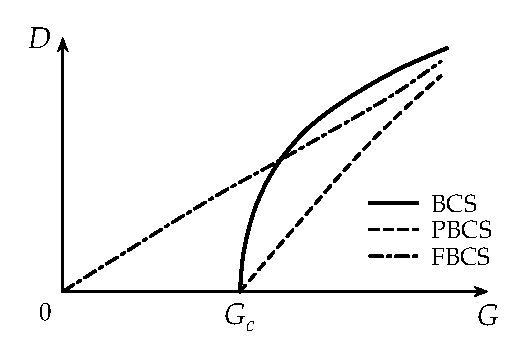
\includegraphics[width=0.55\linewidth]{pictures/11_5}
\par\end{centering}
\centering{}\caption{\label{fig:11_5}BCS（实线）、PBCS（虚线）和FBCS（点虚线）方法中配对关联作为耦合强度 $G$ 的函数（定性）。}
\end{figure}

正如我们在7.7节中所看到的，在这些情况下，我们需要完整的HFB理论，也就是说，我们还必须相对于单粒子波函数 ${\varphi}_{k}$
进行变分。变分后的粒子数投影HFB理论可以通过到目前为止讨论的方法相当简单地得到。由于规范基中的一般HFB波函数（见7.2节）具有BCS函数的结构，我们只需转换到规范基并以相同的方式获得投影矩阵元。

一种避免这些变换的近似方法是基于Fomenko的想法，即将式（11.66）中的积分替换为单位圆上 $L$ 个点 ${\zeta}_{l}=\exp\left({{2\pi il}/L}\right)$
的求和{[}Fo 70, So 72{]}。然后，近似投影算子具有以下形式

\[
{\widehat{P}}^{A}_{L}=\frac{1}{L}\mathop{\sum}\limits^{L}_{{l=1}}{\left({\zeta}_{l}\right)}^{\left({\widehat{N}-A}\right)/2}.\tag{11.74}
\]

很容易看出，除非 $m=0,\pm L,\pm2L,\ldots$，否则 $\widehat{P}^{A+2m}\cdot\widehat{P}^{A}_{L}|\mathrm{BCS}\rangle$
为零。这意味着波函数 $\widehat{P}^{A}_{L}|\mathrm{BCS}\rangle$ 仅包含粒子数 $A,A\pm2L,A\pm4L,\ldots$
的分量。例如，近似投影算符 ${\widehat{P}}^{A}_{2}$ 已经消除了具有 $A\pm2,A\pm6,A\pm{10},\ldots$
的分量。投影后的波函数 $\left({A={2p}}\right)$

\[
{\widehat{P}}^{2p}_{L}|\mathrm{BCS}\rangle=\frac{1}{L}\mathop{\sum}\limits^{L}_{l=1}\zeta^{-p}_{l}\mathop{\prod}\limits_{k>0}\left(u_{k}+v_{k}\zeta_{l}a^{\dagger}_{k}a^{\dagger}_{\bar{k}}\right)|-\rangle\tag{11.75}
\]

是 $L$ 个BCS波函数在规范空间中转动角度 ${\varphi}_{l}={2\pi l}/L$ 后的线性组合；也就是说，
${v}_{k}$ 被替换为 ${e}^{i{\varphi}_{l}}\cdot{v}_{k}$ 。同样， ${\widehat{P}}^{A}_{L}$
将由系数 $\left({{U}_{k{k}^{\prime}},{V}_{k{k}^{\prime}}}\right)$ 给出的HFB函数
$|\Phi\rangle$ 变换为具有系数 $\left({{U}_{k{k}^{\prime}},{\zeta}_{l}{V}_{k{k}^{\prime}}}\right)$
的HFB函数 $\left|{\Phi}_{l}\right\rangle \left({l=1,\ldots,L}\right)$
的线性组合。不需要转换到规范基。

由于BCS波函数仅在少数粒子数上弥散，对于 $L$ 的小值，我们已经得到了近乎精确的投影。

到目前为止，尚未进行粒子数投影后变分的完整HFB理论。无论如何，它比FBCS要复杂得多。在所有实际计算中，使用了依赖于有限数量参数的函数
$|\Phi\left({\beta,\gamma,\Delta}\right)\rangle$ 来最小化投影能量。

\subsection{大形变情况下的近似投影}

Kamlah \cite{Ka68}针对转动群的情况给出了一种在强对称性破缺情况下近似投影的非常通用的方法（另见\cite{Ku72}）。由于转动群表现出许多复杂的特殊特征，并且由于该方法也适用于其他情况，例如粒子数{[}DMR
75, Ma 75a{]}，我们将在此仅针对围绕固定轴的一维转动情况进行介绍。它将由算符 $\widehat{\boldsymbol{J}}$
和角度 $\alpha$ 描述。

投影到 $\widehat{\boldsymbol{J}}$ 的本征函数上的投影算符具有形式（11.57）

\[
{\widehat{P}}^{I}=\frac{1}{2\pi}{\int}^{2\pi}_{0}{e}^{{\mathrm{i}\alpha}\left({\widehat{j}-I}\right)}{\,\mathrm{d}\alpha}\tag{11.76}
\]

对于投影能量，我们得到

\[
{E}^{I}_{\text{ proj }}=\frac{\left\langle \Phi\left|H{\widehat{P}}^{I}\right|\Phi\right\rangle }{\left\langle \Phi\left|{\widehat{P}}^{I}\right|\Phi\right\rangle }=\frac{\int{\,\mathrm{d}\alpha h}\left(\alpha\right){e}^{-{\mathrm{i}I\alpha}}}{\int{\,\mathrm{d}\alpha n}\left(\alpha\right){e}^{-{\mathrm{i}I\alpha}}}\tag{11.77}
\]

带有重叠积分

\[
\left\{ \begin{matrix}h\left(\alpha\right)\\
n\left(\alpha\right)
\end{matrix}\right\} =\langle\Phi\left|{\left\{ \begin{matrix}H\\
1
\end{matrix}\right\} {e}^{{\mathrm{i}\alpha}\widehat{J}}}\right|\Phi\rangle.\tag{11.78}
\]

在粒子数多且变形大的情况下，我们期望函数 $n\left(\alpha\right)$ 和 $h\left(\alpha\right)$
在 $\alpha=0$ 处尖锐地峰值化，而在其他地方消失，使得商 $h\left(\alpha\right)/n\left(\alpha\right)$
是一个相当平滑的函数。这是多体波函数的一个普遍性质（在第10.7节中进行了详细讨论）。遵循第10.7.4节的论证，我们得到\footnote{在以下内容中，我们使用符号 $|\rangle$ 表示归一化的内禀函数 $|\Phi\rangle$。}

\[
n(\alpha)\simeq\exp\left(\mathrm{i}\langle\hat{\boldsymbol{J}}\rangle\cdot\boldsymbol{\alpha}-\frac{1}{2}\langle\Delta\hat{\boldsymbol{J}}^{2}\rangle\alpha^{2}\right),\tag{11.79}
\]

其中

\[
\Delta\widehat{J}=\widehat{J}-\langle\widehat{J}\rangle,
\]

现在唯一的区别是我们也允许波函数中有时间奇数分量，这不会给出纯Gauss分布，而是在式（11.79） $\left({\langle\widehat{J}\rangle\neq0}\right)$
中有一个附加相位。Kamlah的想法是现在使用算符

\[
\widehat{I}\mathrel{\text{ := }}-\langle\widehat{J}\rangle+\frac{1}{i}\frac{\partial}{\partial\alpha},
\]

它是参数 $\alpha$\footnote{对于三维转动的情形，我们因此使用 Euler 角中的角动量表示（见附录 A）来代替 $(1/\mathrm{i})\partial/\partial\alpha$。}
空间中对称算符的一种表示，并以下列方式展开Hamilton重叠函数 $h\left(\alpha\right)$ 。

\[
h\left(\alpha\right)=\mathop{\sum}\limits^{M}_{{n=0}}{h}_{n}{\widehat{I}}^{n}n\left(\alpha\right).\tag{11.80}
\]

从数学上讲，这本质上对应于Fourier变换函数 $h\left(\alpha\right)/n\left(\alpha\right)$
的Taylor展开。由于我们只需要在 $\alpha=0$ 附近的 $h\left(\alpha\right)$ ，如果适当调整，我们已经可以希望用几个非零常数
${h}_{0},{h}_{1},\ldots,{h}_{M}$ 对这个函数得到一个非常好的近似。数字 $M$ 当然取决于重叠（11.79）的宽度，即取决于对称算符
$\widehat{J}$ 在波函数 $|\Phi\rangle$ 中的涨落 $\left\langle {\Delta{\widehat{J}}^{2}}\right\rangle $
。对称性破缺越大，对于低 $M$ 值，近似就越好。

展开式（11.80）不是微扰展开，即系数 ${h}_{n}$ 不是一个接一个地逐步确定，使得系数 ${h}_{0}$ 从 $M$
到 $M+1$ 不会改变，而是对于每个 $M$ 值，整个集合 ${h}_{0},\ldots,{h}_{M}$ 会一次性计算出来：用
$1,\widehat{I},{\widehat{I}}^{2},\ldots,{\widehat{I}}^{M}$ 作用于式（11.80），在极限
$\alpha\rightarrow0$ 下，我们得到关于未知数 ${h}_{0},\ldots,{h}_{M}$ 的如下非齐次方程组：

\[
\left\langle {H{\left(\Delta\widehat{J}\right)}^{m}}\right\rangle =\mathop{\sum}\limits^{M}_{{n=0}}{h}_{n}\left\langle {\left(\Delta\widehat{J}\right)}^{m+n}\right\rangle .\tag{11.81}
\]

这些方程的解为我们给出了投影能量的一个表达式。由（11.77）和（11.80），我们得到

\[
{E}^{I}_{\text{ proj }}=\mathop{\sum}\limits^{M}_{{n=0}}{h}_{n}\cdot{\left(I-\langle\widehat{J}\rangle\right)}^{n}.\tag{11.82}
\]

最简单的情况是 $M=1$ 。在这里我们发现

\[
{h}_{0}=\langle H\rangle,\;{h}_{1}=\frac{\langle{H\Delta}\widehat{J}\rangle}{\left\langle \Delta{\widehat{J}}^{2}\right\rangle },\tag{11.83}
\]

和

\[
{E}^{I}_{\text{ proj }}=\left\langle {\Phi\left|{H-{h}_{1}\widehat{J}}\right|\Phi}\right\rangle +{h}_{1}\cdot I.\tag{11.84}
\]

在投影方法之后的一种变分方法中，我们得到变分方程

\[
\frac{\delta}{\delta\Phi}\langle\Phi\left|H\right|\Phi\rangle-{h}_{1}\frac{\delta}{\delta\Phi}\langle\Phi\left|\widehat{J}\right|\Phi\rangle+\left({I-\langle\widehat{J}\rangle}\right)\frac{\delta{h}_{1}}{\delta\Phi}=0.\tag{11.85}
\]

它由推转方程的一个解来满足\footnote{在某些情况下，该解并非对应于极小值，而是对应于平坦的极大值。然而，二阶项（$M=2$）保证了该极大值变为极小值 \cite{BMR70}（另见第
11.4.6 节）。}：

\[
\frac{\delta}{\delta\Phi}\langle\Phi|H|\Phi\rangle-\omega\frac{\delta}{\delta\Phi}\langle\Phi|\hat{J}|\Phi\rangle=0,\tag{11.86}
\]

和

\[
\langle\widehat{J}\rangle=I
\]

如果条件 ${h}_{1}=\omega$ 得到满足。为了证明情况总是如此，我们利用这样一个事实，即对于直积波函数集合中的任意变分
$|{\delta\Phi}\rangle$ ，式（11.86）都必须成立。其中一种变分由 $|\delta\Phi\rangle\propto\Delta\widehat{J}|\Phi\rangle=\widehat{J}^{20}|\Phi\rangle$（在第7章准粒子表象的意义下）给出。因此，我们得到

\[
\langle\Delta\widehat{J}H\rangle-\omega\left\langle {\left(\Delta\widehat{J}\right)}^{2}\right\rangle =0,
\]

这表明式（11.83）中的 $\omega={h}_{1}$ 。

我们现在已经证明了一个显著的结果，即在强对称性破缺的情况下，当 $M=1$ 在展开式（11.80）中是一个足够好的近似时，保持平均对称性的转动模型波函数是投影后变分方程的一个解。这个结果并不详细依赖于重叠函数的结构。只需要它们在原点附近有尖锐的峰值这一事实。

到目前为止，我们仅在一维转动的情况下证明了这一点，但结果（正如我们将在第11.4.4节中看到的）只需稍作修改，也可应用于三维情况。

在这种近似下，投影能量由 ${h}_{0}$ 给出，且等于未投影能量。这证明了转动谱的自洽转动模型计算是合理的（见第 7.7 节）。特别地，对于自洽转动惯量，我们发现

\[
{g}^{-1}_{\mathrm{{sc}}}=\frac{\omega}{\langle\widehat{J}\rangle}=\frac{\langle{H\Delta}\widehat{J}\rangle}{\left\langle {\Delta{\widehat{J}}^{2}}\right\rangle \langle\widehat{J}\rangle}.\tag{11.87}
\]

如8.5.4节所讨论的，在 $\omega=0$ 点它与Thouless和Valatin的点相同。

然而，这个简单的结果仅适用于能量期望值。如果我们想要计算矩和跃迁概率，就必须从内禀转动函数进行显式投影（见第11.4.6.4节）。

在展开式（11.80）中对 $M=1$ 的限制不够好的情况下，我们必须采用更高的 $M$ 值。对于 $M=2$，我们忽略\footnote{$\langle\Delta\hat{J}^{3}\rangle$ 测量了 $|\Phi\rangle$ 中 $I$ 分布的不对称性。在
Gauss 模重叠的情况下，它精确为零。} $\langle\Delta\hat{J}^{3}\rangle$，并得到

\[
{h}_{0}=\langle H\rangle-\frac{\left\langle \Delta{\widehat{J}}^{2}\right\rangle }{2{\mathcal{G}}_{Y}},\;{h}_{1}=\frac{\left\langle H\Delta\widehat{J}\right\rangle }{\left\langle \Delta{\widehat{J}}^{2}\right\rangle }=\frac{\left\langle \widehat{J}\right\rangle }{{\mathcal{G}}_{\mathrm{{sc}}}},\;{h}_{2}=\frac{1}{2{\mathcal{G}}_{Y}},\tag{11.88}
\]

其中

\[
\frac{1}{2{g}_{Y}}=\frac{\left\langle {{H\Delta}{\widehat{J}}^{2}}\right\rangle -\langle H\rangle\left\langle {\Delta{\widehat{J}}^{2}}\right\rangle }{\left\langle {\Delta{\widehat{J}}^{4}}\right\rangle -{\left\langle \Delta{\widehat{J}}^{2}\right\rangle }^{2}}.\tag{11.89}
\]

在Gauss范数（11.79）的情况下，我们有 $\left\langle {\Delta{\widehat{J}}^{4}}\right\rangle =3{\left\langle \Delta{\widehat{J}}^{2}\right\rangle }^{2}$
并发现

\[
{g}^{-1}_{Y}=\frac{\left\langle \left(H-\langle H\rangle\right)\Delta{\widehat{J}}^{2}\right\rangle }{{\left\langle \Delta{\widehat{J}}^{2}\right\rangle }^{2}}.\tag{11.90}
\]

投影后的能量现在具有以下形式：

\[
{E}^{I}_{\text{ proj }}=\langle H\rangle-\frac{\left\langle \Delta{\widehat{J}}^{2}\right\rangle }{2{g}_{Y}}+\frac{\left\langle \widehat{J}\right\rangle }{{g}_{\mathrm{{sc}}}}\left({I-\langle\widehat{J}\rangle}\right)+\frac{1}{2{g}_{Y}}{\left(I-\langle\widehat{J}\rangle\right)}^{2}.\tag{11.91}
\]

让我们首先研究投影前的变分方法，这最初是由Peierls和Yoccoz{[}PY 57, Yo 57{]}提出的。这里，波函数 $|\Phi\rangle$
是通过在无约束条件下最小化 $H$ 得到的。因此，它是时间反演不变的，并且期望值 $\langle\widehat{J}\rangle$
和 $\langle H\widehat{J}\rangle$ 为零。然后，能谱具有以下形式

\[
{E}^{I}_{\text{ proj }}=\left\langle {H-\frac{{\widehat{J}}^{2}}{2{g}_{Y}}}\right\rangle +\frac{{I}^{2}}{2{g}_{Y}}.\tag{11.92}
\]

它是一个一维转子的能谱，其转动惯量为Yoccoz值 $\mathcal{J}_{Y}$ （见第11.4.5节）\footnote{Verhaar \cite{Ve63,Ve64} 也针对偶核和奇核中 $K=0$ 和 $K\neq0$ 带的三维转动详细研究了该方法。因此人们可以推导出式（3.1）中
$B$ 和 $C$ 系数以及退耦参数（3.31）的微观表达式。}。带首能量是通过从 HF 能量 $\langle H\rangle$ 中减去对称破缺波函数中的赝转动能量得到的\footnote{关于此贡献的计算，见 \cite{ZN77,VLS79,ER80}。}。这使得基态能量大幅降低。在形变良好的原子核中，这个项的量级为4
- 6 MeV。我们已经在几个例子中遇到过这个项，例如，在冗余坐标方法（见第11.3.2节）以及RPA方法中对对称破缺处理（第8.4.8节）。

进行投影后的变分，我们必须相对于 $|\Phi\rangle$ 最小化式（11.91）的右侧。在赝能量 $\left\langle {\Delta{\widehat{J}}^{2}}\right\rangle /2{\mathcal{J}}_{Y}$
不太依赖于 $|\Phi\rangle$ 的情况下，我们再次发现转动模型是一个解。稀土区域形变良好的原子核的模型计算\cite{BMR70}表明，这个项确实对能量曲面给出了相当平坦的贡献。

坎拉展开式（11.80）的收敛性取决于重叠函数在原点处的峰值尖锐程度。它由宽度 $\left\langle {\Delta{\widehat{J}}^{2}}\right\rangle $
衡量，也就是由对称算符的涨落衡量。如果这个涨落很大，展开式收敛很快。我们称这种情况为大形变极限，并且我们想要强调这个极限不一定与相应平均场中的大形变参数相关。在粒子数很大的情况下，即使形变参数很小，涨落
$\left\langle {\Delta{\widehat{J}}^{2}}\right\rangle $ 也可能有很大的值。实际上，基态下“形变良好”的重核形状与球体并没有太大差别（例如，见图7.5）。然而，由于粒子数很大，重叠函数在原点处强烈峰值化，这表明向形变平均场的相变假设是合理的。

\subsection{惯性参数}

在所有与连续对称性破缺相关的集体运动中，势能 $\langle H\rangle$ （11.9） 不依赖于集体坐标。因此，不存在恢复力，并且在大多数转动类型的情况下，我们总是得到大振幅的运动。因此，集体Hamilton量的关键参数是惯性参数。

有一种情况我们可以先验地知道这个参数：由于伽利略不变性，平移的集体惯性必须等于系统的总质量 ${Am}$ 。因此，这种情况为迄今为止在处理对称性破缺时使用的不同近似方案提供了一个非常好的检验。

我们从投影后变分法开始{[}Ze 65, Vi 66, RY 66{]}。方程（11.62）定义了具有动量p的波函数的本征解：

\[
\langle{\delta\Phi}\left|{\left({H-{E}^{\boldsymbol{p}}}\right){\widehat{P}}^{\boldsymbol{p}}}\right|\Phi\rangle=0.\tag{11.93}
\]

从实验室系统变换到以速度 $\boldsymbol{v}=\boldsymbol{p}/{2Am}$ 运动的系统，我们发现（ $\boldsymbol{R}$
是质心坐标）：

\[
|\Phi\rangle={e}^{(\mathrm{i}/\hbar)\boldsymbol{p}\cdot\boldsymbol{R}}|{\Phi}^{\prime}\rangle\tag{11.94}
\]

和

\[
\left\langle {\delta{\Phi}^{\prime}\left|{{e}^{-\left({\mathrm{i}/\hbar}\right)\boldsymbol{p}\boldsymbol{R}}\left({H-{E}^{\boldsymbol{p}}}\right){\widehat{P}}^{\boldsymbol{p}}{e}^{\left({\mathrm{i}/\hbar}\right)\boldsymbol{p}\boldsymbol{R}}}\right|{\Phi}^{\prime}}\right\rangle =0.\tag{11.95}
\]

使用投影仪 ${\widehat{P}}^{\mathrm{p}}$ 的定义（11.59），我们得到变换

\[
{e}^{-\left({\mathrm{i}/\hbar}\right)\boldsymbol{p}\boldsymbol{R}}{\widehat{P}}^{\boldsymbol{p}}{e}^{\left({\mathrm{i}/\hbar}\right)\boldsymbol{p}\boldsymbol{R}}={\widehat{P}}^{\boldsymbol{0}}.\tag{11.96}
\]

对于局部两体相互作用，我们得到

\[
{e}^{-\left({\mathrm{i}/\hbar}\right)\boldsymbol{p}\boldsymbol{R}}H{e}^{\left({\mathrm{i}/\hbar}\right)\boldsymbol{p}\boldsymbol{R}}=H+\frac{\boldsymbol{{pP}}}{Am}+\frac{{\boldsymbol{p}}^{2}}{2Am}.\tag{11.97}
\]

由于 ${\widehat{P}}^{0}$ 投影到质心动量 $\boldsymbol{P}$ 的本征值为零的态上，式（11.95）具有如下形式

\[
\left\langle {\delta{\Phi}^{\prime}\left|{\left({H-{E}^{\mathrm{p}}+\frac{{\boldsymbol{p}}^{2}}{2Am}}\right){\widehat{P}}^{0}}\right|{\Phi}^{\prime}}\right\rangle =0.\tag{11.98}
\]

它对应于动量和能量 ${E}^{0}$ 消失时的变分问题。因此，具有动量 $\boldsymbol{p}$ 的系统的能量由下式给出

\[
{E}^{\mathrm{p}}={E}^{0}+\frac{{\boldsymbol{p}}^{2}}{2Am},\tag{11.99}
\]

这表明我们在变分后使用投影方法获得了正确的总质量。如果我们通过自洽转动模型\cite{Gr60}（在平移的情况下，我们通常说“推”模型）来近似变分后的投影，这个性质是守恒的：

\[
\langle{\delta\Phi}\left|{H-\boldsymbol{v}\boldsymbol{P}}\right|\Phi\rangle=0.\tag{11.100}
\]

通过这种方式得到的Thouless和Valatin的惯性参数（8.113）就是总质量。原则上，我们在8.4.7节中已经证明了这一点，但如果我们使用允许的变分，很容易再次验证它

\[
|\delta\Phi\rangle\propto\boldsymbol{R}|\Phi\rangle.\tag{11.101}
\]

用式（11.100）的复共轭减去它本身，我们得到

\[
\langle\Phi\left|{\left\lbrack {H,\boldsymbol{R}}\right\rbrack -\boldsymbol{v}\cdot\left\lbrack {\boldsymbol{P},\boldsymbol{R}}\right\rbrack }\right|\Phi\rangle=0.\tag{11.102}
\]

在仅包含局部两体相互作用的 $H$ 情况下，我们得到

\[
\boldsymbol{v}=\frac{\langle\Phi\left|\boldsymbol{P}\right|\Phi\rangle}{Am},\tag{11.103}
\]

这表明，由 $\boldsymbol{P}$ 的期望值与速度 $\boldsymbol{v}$ 的比值给出的惯性参数再次是总质量。

如果我们将Hamilton量 $H$ 中的两体相互作用替换为单体势（在这种情况下变分原理等同于精确对角化），那么我们也可以从变分方程（11.93）推导出简单的Inglis公式{[}见式（3.89）{]}作为惯性参数。这向我们表明，对于局部单体势，例如对于
Woods-Saxon 势阱，Inglis 公式也给出了精确的总质量\footnote{这与 Thouless-Valatin 质量（8.113）由于剩余相互作用而与 Inglis 公式不同的事实并不矛盾，因为对于产生局域
HF 场的所有力，剩余相互作用对质量没有影响（式（12.81）中的时间奇部分 $\Gamma_{1}$ 消失）。} \cite{Vi63}。

投影前变分法的一个缺点是它违反了伽利略不变性，该方法得出了Yoccoz\footnote{内禀波函数 $|\Phi\rangle$ 是转动带所有成员 $\Psi^{I}$ 的叠加这一思想也被 Skyrme \cite{Sk57}
使用过：假设内禀 Hamilton 量 $H'=H-\boldsymbol{J}^{2}/2\mathcal{J}$ 具有一个本征态，该本征态不是
$\boldsymbol{J}^{2}$ 的本征态，我们可以证明 \cite{Li60a} $H$ 具有以 $\mathcal{J}$
为转动惯量的转动能谱。为了确定 $\mathcal{J}$ 的最优值，Skyrme 针对参数 $\mathcal{J}$ 最小化期望值
$\langle(H'-\langle H'\rangle)^{2}\rangle$，并找到如下解：
\[
\frac{1}{2\mathcal{J}_{\text{Skyrme}}}=\frac{\langle(H-\langle H\rangle)\boldsymbol{J}^{2}\rangle}{\langle\boldsymbol{J}^{4}\rangle-\langle\boldsymbol{J}^{2}\rangle^{2}}.
\]
对于时间偶波函数，此表达式与式（11.89）完全相同，因此与 $\mathcal{J}_{Y}$ 紧密相关（另见 \cite{Wo75}）。} 的惯性（11.90）。它不能产生精确的质量。从方程（11.90）和（10.134）中，我们用8.4.7节的符号表示法得到惯性（另见\cite{FW70}）：

\[
{g}^{-1}_{Y}=\frac{1}{4{\left\langle \Delta{P}^{2}\right\rangle }^{2}}{\left\langle {\left\lbrack P,{\left\lbrack H,P\right\rbrack }_{+}\right\rbrack }_{+}\right\rangle }_{L}=\frac{\left({{P}^{*}P}\right)\left(\begin{matrix}A & B\\
{B}^{*} & {A}^{*}
\end{matrix}\right)\left(\begin{matrix}P\\
{P}^{*}
\end{matrix}\right)}{{\left(2\mathop{\sum}\limits_{{mi}}{\left|{P}_{mi}\right|}^{2}\right)}^{2}},\tag{11.104}
\]

其中，如果使用自洽基 $\left({{H}^{20}=0}\right)$ ，则 $P$ 是矢量 $\boldsymbol{P}$
的一个分量的 ${ph}$ 部分。在残余相互作用消失的极限情况下，它等于

\[
{\mathcal{I}}_{Y}\left({V=0}\right)=\frac{2{\left(\mathop{\sum}\limits_{{mi}}{\left|{P}_{mi}\right|}^{2}\right)}^{2}}{\mathop{\sum}\limits_{{mi}}{\left|{P}_{mi}\right|}^{2}\left({{\epsilon}_{m}-{\epsilon}_{i}}\right)}.\tag{11.105}
\]

它显然与 Thouless - Valatin 惯性（8.108）不同，

\[
{g}^{-1}_{\mathrm{{TV}}}=\frac{1}{{\hbar}^{2}}\left\langle {\left\lbrack R,{\left\lbrack H,R\right\rbrack }_{-}\right\rbrack }_{-}\right\rangle =\frac{2}{{\hbar}^{2}}{S}_{1}\left(R\right)
\]

or

\[
{g}_{\mathrm{{TV}}}=\frac{1}{2}\left({{P}^{*}P}\right){\left(\begin{array}{ll}
A & B\\
{B}^{*} & {A}^{*}
\end{array}\right)}^{-1}\left(\begin{array}{l}
P\\
{P}^{*}
\end{array}\right)\tag{11.106}
\]

在相互作用消失的极限情况下，它会过渡到 Inglis 公式（3.89），

\[
\mathcal{J}^{-1}_{\text{TV}}(V=0)=2\sum_{mi}\frac{|P_{mi}|^{2}}{\epsilon_{m}-\epsilon_{i}}.\tag{11.107}
\]

这种差异实际上有多大以及有多重要，尚未得到充分研究。它肯定取决于相互作用和单粒子能量 ${\epsilon}_{k}$ 。对于所有具有恒定能级间距
$\epsilon={\epsilon}_{m}-{\epsilon}_{i}$ 的模型，这两个值是相同的。在第 10.7 节中我们看到，如果我们使用具有坐标依赖生成函数的简单
GCM 方法，对于各种集体运动我们都有 Yoccoz 惯性（11.104）。只有在我们允许本征函数 $|\Phi\rangle$
也具有依赖于动量的时间奇数分量的理论中，我们最终才能得到正确的质量。在含时 Hartree - Fock 方法（见第 12 章）和投影后变分方法中就是这种情况。

为了在 GCM 方法中也得到正确的质量，Thouless 和 Peierls \cite{PT62} 提议不仅叠加不同位置的波函数
{[}见式（11.59）{]}，

\[
|\Phi(\boldsymbol{q})\rangle={e}^{(\mathrm{i}/\hbar)\boldsymbol{q}\cdot\boldsymbol{P}}|\Phi\rangle,\tag{11.108}
\]

而且叠加不同速度的波函数，

\[
|\Phi(\boldsymbol{q},\boldsymbol{v})\rangle=e^{-(\mathrm{i}/\hbar)M\boldsymbol{v}\cdot\boldsymbol{R}}|\Phi(\boldsymbol{q})\rangle.\tag{11.109}
\]

这产生了一种双投影方法，其中权重函数 $f\left({\boldsymbol{q},\boldsymbol{v}}\right)$
的速度依赖性必须通过变分来确定。我们可以证明以这种方式得到的波函数不违反伽利略不变性。然而，该方法本身相当复杂，到目前为止尚未得到广泛应用
\cite{Ba69b}。在实际计算中，通常更喜欢投影后变分方法（见第 11.4.2 节）。

到目前为止，我们只处理了平移的情况。在第 10.7 节中讨论的转动或其他集体运动的情况下，情况更为复杂。精确的转动惯量事先并不知道。我们只能类比平移的情况进行论证。数值计算至少表明，在转动情况下，通过
Thouless 和 Valatin 方法得到的转动惯量，在适当处理配对关联的情况下，与实验数据吻合得很好（见图 3.14）。

\subsection{角动量投影}

\subsubsection{类投影算符的推导}

转动群通常由三个 Euler 角\footnote{也使用过其他表示，例如对于参数为 $\varphi_{x},\varphi_{y},\varphi_{z}$ 的一般转动使用 $R=\exp(\mathrm{i}\boldsymbol{\varphi}\cdot\hat{\boldsymbol{J}})$
\cite{KO77}。} $\Omega=\left({\alpha,\beta,\gamma}\right)$ 参数化，一般转动由式（A.4）给出。我们必须回到波函数
$|\Psi\rangle$ 的假设式（11.53）。如同式（11.55），我们将权重函数 $f\left(\Omega\right)$
展开为相应对称算符的一组完备本征函数：用Euler角表示的角动量。如附录A中所讨论的，这样一组函数由Wigner函数 ${D}^{{I}^{*}}_{MK}\left(\Omega\right)$
给出。因此我们得到假设式

\[
f\left(\Omega\right)=\frac{{2I}+1}{8{\pi}^{2}}\mathop{\sum}\limits_{{IMK}}{g}_{IMK}{D}^{{I}^{*}}_{MK}\left(\Omega\right)\tag{11.110}
\]

以及

\[
|\Psi\rangle=\mathop{\sum}\limits_{IMK}g_{IMK}\widehat{P}^{I}_{MK}|\Phi\rangle.\tag{11.111}
\]

算符{[}RW 54, PY 57, Vi 66{]}

\[
{\widehat{P}}^{I}_{MK}=\frac{{2I}+1}{8{\pi}^{2}}\int{D}^{{I}^{*}}_{MK}\left(\Omega\right)R\left(\Omega\right){\,\mathrm{d}\Omega}\tag{11.112}
\]

\[
R\left(\Omega\right)={e}^{{\mathrm{i}\alpha}{\widehat{J}}_{z}}{e}^{{\mathrm{i}\beta}{\widehat{J}}_{y}}{e}^{{\mathrm{i}\gamma}{\widehat{J}}_{z}}
\]

可以类似于式（11.58）那样书写{[}LB 68, Co 71{]}

\[
\widehat{P}^{I}_{MK}=\mathop{\sum}\limits_{\alpha}|IM\alpha\rangle\langle IK\alpha|,\tag{11.113}
\]

其中 $|{IM\alpha}\rangle$ 是希尔伯特空间中的一组完备正交归一化函数集， $\alpha$ 除了转动量子数
$I$ 和 $M$ 之外还表征所有量子数。

从式（11.113）我们看到 ${\widehat{P}}^{I}_{MK}$ 在数学意义上不是投影算符。我们只有以下关系

\[
{\widehat{P}}^{I}_{MK}{\widehat{P}}^{{I}^{\prime}}_{{M}^{\prime}{K}^{\prime}}={\delta}_{I{I}^{\prime}}{\delta}_{{M}^{\prime}K}{\widehat{P}}^{I}_{M{K}^{\prime}};\;\left({\widehat{P}}^{I}_{MK}\right)^{\dagger}={\widehat{P}}^{I}_{KM}.\tag{11.114}
\]

为了展示它们如何相对于具有量子数 $K$ 的算符 ${\widehat{J}}_{z}$ 的本征态作用于“内秉”\footnote{实际上，在 GCM 方法中我们既不引入内秉参考系也不引入冗余坐标。“内秉”波函数 $|\Phi\rangle$ 与实验室参考系中的函数
$|\Psi\rangle$ 之间的联系不是由坐标变换给出，而是由 GCM 假设式（11.111）给出。}违反对称性的波函数$|\Phi\rangle$，我们将 $|\Phi\rangle$ 分解为：

\[
|\Phi\rangle=\mathop{\sum}\limits_{K'}|\Phi_{K'}\rangle;\quad\widehat{J}_{z}|\Phi_{K}\rangle=K|\Phi_{K}\rangle.\tag{11.115}
\]

${\widehat{P}}^{I}_{MK}$ 将分量 $\left|{\Phi}_{K}\right\rangle $ 变换为具有量子数
$I$ 和 $M$ 的 ${\widehat{\boldsymbol{J}}}^{2}$ 和 ${\widehat{J}}_{z}$
的本征函数，并使所有其他具有 ${K}^{\prime}\neq K$ 的分量湮灭。

原则上，构造到量子数 $I,M$ 上的精确数学投影算符非常简单。它由\footnote{这个算符已由 Löwdin \cite{Lo64} 以如下方式表示：
\[
\hat{P}^{I}_{MM}=\prod_{L\neq I}\frac{\hat{\boldsymbol{J}}^{2}-L(L+1)}{I(I+1)-L(L+1)}\prod_{K\neq M}\frac{\hat{J}_{z}-K}{M-K}.
\]
在这个算符的实际应用中，我们最终得到一组代数方程（另见 \cite{KL64,Ke66,Ul71,Ul72,MKL71,MM76}），并且不必对
Euler 角进行积分。}给出

\[
\widehat{P}^{I}_{MM}=\mathop{\sum}\limits_{\alpha}|IM\alpha\rangle\langle IM\alpha|.\tag{11.116}
\]

然而，从式（11.115）我们看到这个算符相当不物理。例如，作用于具有 $K=0$ 的轴对称Nilsson函数上，我们只会得到具有
$M=0$ 的波函数 $\left|{\Psi}^{IM}\right\rangle $ ，这显然违反了转动对称性。

因此我们必须使用一般拟设\footnote{正如我们从式（11.120）中看到的，系数 $g_{K}$ 当然也依赖于 $I$。然而，我们省略了指标 $I$。}

\[
|\Psi^{IM}\rangle=\mathop{\sum}\limits_{K}g_{K}\widehat{P}^{I}_{MK}|\Phi\rangle=\mathop{\sum}\limits_{K}g_{K}\frac{2I+1}{8\pi^{2}}\int\,\mathrm{d}\Omega\,D^{I*}_{MK}(\Omega)R(\Omega)|\Phi\rangle.\tag{11.117}
\]

在波函数 $|\Phi\rangle$ 具有轴对称性的情况下，只有 $K$ 值 ${K}_{0}$ 对总和（11.117）有贡献，并且系数
${g}_{{K}_{0}}$ 由归一化给出。然而，一般来说，我们必须相对于系数 ${g}_{K}$ 使Hamilton量最小化。能量由下式给出

\[
{E}^{I}_{\text{ proj }}=\frac{\left\langle {\Psi}^{IM}\left|H\right|{\Psi}^{IM}\right\rangle }{\left\langle {\Psi}^{IM}\mid{\Psi}^{IM}\right\rangle }=\frac{\mathop{\sum}\limits_{{K{K}^{\prime}}}{g}^{*}_{K}{g}_{{K}^{\prime}}{h}^{I}_{K{K}^{\prime}}}{\mathop{\sum}\limits_{{K{K}^{\prime}}}{g}^{*}_{K}{g}_{{K}^{\prime}}{n}^{I}_{K{K}^{\prime}}},\tag{11.118}
\]

以及核

\[
h^{I}_{KK'}=\langle\Phi|H\hat{P}^{I}_{KK'}|\Phi\rangle,
\]

\[
n^{I}_{KK'}=\langle\Phi|\hat{P}^{I}_{KK'}|\Phi\rangle.\tag{11.119}
\]

系数 ${g}_{K}$ 是广义特征值问题的解

\[
\mathop{\sum}\limits_{{K}^{\prime}}{h}^{I}_{K{K}^{\prime}}{g}_{{K}^{\prime}}={E}^{I}\mathop{\sum}\limits_{{K}^{\prime}}{n}^{I}_{K{K}^{\prime}}{g}_{{K}^{\prime}}.\tag{11.120}
\]

它对应于Hamilton量 $H$ 在由非正交系统 ${\widehat{P}}^{I}_{MK}|\Phi\rangle$ 所张成空间中的对角化。

在第10.7节中，我们看到了如何进行操作以便最终得到一个厄米特特征值问题。我们必须要么将集合 ${\widehat{P}}^{I}_{MK}|\Phi\rangle$
正交化，要么计算矩阵 ${n}^{I}_{K{K}^{\prime}}$ 的平方根。在重叠函数 $\langle\Phi\left|{R\left(\Omega\right)}\right|\Phi\rangle$
为Gauss形式的情况下，也就是说，对于一个强变形波函数（见第11.4.4节），我们可以解析地做到这一点。由于我们面临的是一个三维问题，最终会得到一个像式（10.145）那样的集体Hamilton量。Une等人\cite{UIO76}已经表明，它具有转子Hamilton量（1.55）的精确形式，其转动惯量由Yoccoz公式\footnote{另见 \cite{ABC77a}。}
给出（见第11.4.5节）。

如果我们定义极其变形的多体波函数\footnote{这些函数对应于式（10.20）及后续讨论的双正交基。}
$|\Omega\rangle$ ，它在方向 $\Omega$ 上像针一样指向，那么与集体转子模型的紧密类比就很容易可视化。它们在
$\Omega$ 空间中几乎是局域化的。这些函数与波函数 $\left|{\Psi}^{IM}\right\rangle $ （11.117）之间的重叠

\[
\langle\Omega|{\Psi}^{IM}\rangle\propto\mathop{\sum}\limits_{K}\;{g}_{K}\int d{\Omega}^{\prime}\;{D}^{{I}^{*}}_{MK}\left({\Omega}^{\prime}\right)\langle\Omega|R\left({\Omega}^{\prime}\right)|\Phi\rangle,\tag{11.121}
\]

测量在角度 $\Omega$ 处找到系统的概率幅。在波函数 $|\Phi\rangle$ 充分变形且在 $\Omega=0$
处达到峰值的极限情况下，重叠 $\left\langle {\Omega\left|{R\left({\Omega}^{\prime}\right)}\right|\Phi}\right\rangle $
在 $\Omega$ 空间中的行为类似于 $\delta$ 函数 $\delta\left({\Omega-{\Omega}^{\prime}}\right)$
，并且我们得到{[}Ze 67, FJM 71{]}

\[
\langle\Omega|\Psi^{IM}\rangle\propto\sum_{K}g_{K}D^{I*}_{MK}(\Omega)\tag{11.122}
\]
\footnote{【译者注】也使用过其他表示，例如 $R=\mathrm{e}^{-\mathrm{i}\alpha J_{z}}\mathrm{e}^{-\mathrm{i}\beta J_{y}}\mathrm{e}^{-\mathrm{i}\gamma J_{z}}$
；此时 $D$ 函数与 Edmonds \cite{Ed57} 的相符合。我们在这里使用的定义（11.118）与 Rose \cite{Ro57}
的相符合。}

这正是一个转子的波函数（见第1.5.1节）。在这种近似下，变形函数 $|\Phi\rangle$ 在空间中像转子一样运动。然而，我们必须强调，我们没有使用冗余变量。Euler角
$\Omega$ 仅仅是用作生成坐标的参数。

与转子的对称行为类似，在群 ${D}_{2}$ 的某些操作下{[}例如，式（1.57）及后续中的 ${\Re}_{1}$ 或 ${\Re}_{2}$
{]}会导致展开系数 ${g}^{\left(\text{ rotor }\right)}_{K}$ 之间的关系，现在如果我们的内部波函数具有这些对称性，我们就可以为系数
${g}_{K}$ 推导相应的关系。

作为一个例子，我们使用 ${180}^{\circ}$ 绕 $x$ 轴的转动。我们假设\footnote{这一假设与我们方法的转动不变性是相容的，因为内部波函数 $|\Phi\rangle$ 绕 Euler 角 $\Omega$ 的转动可以表示为系数
$g_{K}$ 的变换，正如我们从关系式
\[
\hat{P}^{I}_{MK}R(\Omega)=\sum_{K'}D^{I}_{KK'}(\Omega)\hat{P}^{I}_{MK'}\tag{11.123}
\]
中所看到的。只要我们考虑任意系数 $g_{K}$，我们就可以自由选择 $|\Phi\rangle$ 的取向。}内部波函数 $|\Phi\rangle$ 关于此操作是一个本征函数：

\[
{e}^{\mathrm{i}\pi{\widehat{J}}_{x}}|\Phi\rangle={r}_{x}|\Phi\rangle.\tag{11.124}
\]

对于粒子数为偶数的系统，本征值 ${r}_{x}$ 为 $\pm1$ ；对于粒子数为奇数的系统，本征值为 $\pm i$ 。它常被称为signature
\cite{Bo76b}。例如，在变形的Nilsson势阱中，偶偶核的基态总是具有 ${r}_{x}=+1$ ，因为以 $\pm i$
成对占据简并能级会给出最低能量。因此，基态带的 ${r}_{x}=+1$ 条件是变分原理的自然结果。这一事实为转子模型的假设（1.58）提供了微观基础——即变形核相对于操作
${\Re}_{1}$ （1.57）具有本征值 +1。

对称性（11.123）相当普遍，也适用于转动模型波函数。到目前为止，尚未发现它无效的实验证据。因此，我们将在以下内容中使用这种对称性。

如果我们像在式（11.115）中那样，将内部波函数 $|\Phi\rangle$ 分解为具有良好 $K$ 量子数的分量 $\left|{\Phi}_{K}\right\rangle $
，那么从（11.123）可得：

\[
{e}^{{\mathrm{i}\pi}{\widehat{J}}_{x}}\left|{\Phi}_{K}\right\rangle ={r}_{x}\left|{\Phi}_{-K}\right\rangle .\tag{11.125}
\]

从式（11.124）我们可以推断出

\[
{\widehat{P}}^{I}_{MK}{e}^{{\mathrm{i}\pi}{\widehat{J}}_{x}}={\left(-\right)}^{I}{\widehat{P}}^{I}_{MK},\tag{11.126}
\]

这表明态

\[
\widehat{P}^{I}_{MK}|\Phi\rangle=\widehat{P}^{I}_{MK}|\Phi_{K}\rangle\quad\text{以及}\quad\widehat{P}^{I}_{M-K}|\Phi\rangle=\widehat{P}^{I}_{M-K}|\Phi_{-K}\rangle
\]

在希尔伯特空间中对应于同一态。因此，我们可以限制式（11.117）中对 $K\geq0$ 的求和。\footnote{【译者注】正如我们从式（11.120）中看到的，系数 $a_{M}$ 仅由实验室系统中的边界条件决定（例如磁量子数 $M$ 
的指定）。对于孤立核，所有 $M$ 
态简并，我们通常只考虑 $a_{M}=\delta_{MM_{0}}$ 的情形。}

表示

\[
\left|{\Psi}^{IM}\right\rangle =\mathop{\sum}\limits_{{K>0}}\frac{{g}_{K}}{1+{\delta}_{K0}}\left({{\widehat{P}}^{I}_{MK}+{\left(-\right)}^{I}{r}^{-1}_{x}{\widehat{P}}^{I}_{M-K}}\right)|\Phi\rangle\tag{11.127}
\]

清楚地表明，对于奇数 $I$ 值，具有 $K=0$ 和 ${r}_{x}=1$ 的轴对称波函数 $|\Phi\rangle$
投影为零。因此，对于基态带，我们得到自旋序列 $I=0,2,4,\ldots$

在我们只有近似轴对称的情况下，如在转动模型波函数中（见7.7节和11.4.6.3节），剩余的 $K\neq0$ 部分不会投影为零。然而，它们源于两准粒子态和更复杂构型的混合，这些混合处于更高能量，并且仅对本征值问题（11.120）中的高激发能级有贡献，而我们对此并不感兴趣。因此，对于基态带，我们应该施加条件

\[
{r}_{x}={\left(-\right)}^{I}.\tag{11.128}
\]


\subsubsection{双变分法\label{subsec:=0053CC=0053D8=005206=006CD5}}

到目前为止，我们尚未指定确定内禀波函数 $|\Phi\rangle$ 的方法。与11.4.2节中讨论的阿贝尔群的情况一样，我们可以在投影之前或之后进行变分。然而，在没有轴对称的情况下，情况现在更复杂了，因为我们还必须确定系数
${g}_{K}$ 。在VBP方法中，它们必须通过式（11.120）计算。

在VAP方法中，我们现在得到一个类似于系统（10.147） \cite{Ze67}的耦合系统：

\[
\mathop{\sum}\limits_{{K}^{\prime}}{g}_{{K}^{\prime}}\left\langle {\Phi\left|{\left({H-{E}^{I}}\right){\widehat{P}}^{I}_{K{K}^{\prime}}}\right|\Phi}\right\rangle =0
\]

\[
\mathop{\sum}\limits_{{K{K}^{\prime}}}{g}^{*}_{K}{g}_{{K}^{\prime}}\left\langle {{\delta\Phi}\left|{\left({H-{E}^{I}}\right){\widehat{P}}^{I}_{K{K}^{\prime}}}\right|\Phi}\right\rangle =0.\tag{11.129}
\]

第一部分对应于式（11.120）；第二部分是VAP方程（11.62）的推广。原则上，这个系统必须通过迭代求解。

除了系统（11.129）过于复杂以至于无法精确求解这一事实外，在许多情况下它还包含高度的冗余性。为了看到这一点，我们再次使用 $|\Phi\rangle$
分解为各 $K$ 分量的式（11.115）。利用 ${\widehat{P}}^{I}_{MK}$ 使所有 $K\neq{K}^{\prime}$
的 $\left|{\Phi}_{{K}^{\prime}}\right\rangle $ 分量湮灭这一事实，我们得到

\[
\left|{\Psi}^{IM}\right\rangle =\mathop{\sum}\limits_{K}{\widehat{P}}^{I}_{MK}\mathop{\sum}\limits_{{K}^{\prime}}{g}_{{K}^{\prime}}\left|{\Phi}_{{K}^{\prime}}\right\rangle =\mathop{\sum}\limits_{K}{\widehat{P}}^{I}_{MK}|\widetilde{\Phi}\rangle.\tag{11.130}
\]

函数

\[
|\widetilde{\Phi}\rangle=\mathop{\sum}\limits_{K}{g}_{K}|{\Phi}_{K}\rangle\tag{11.131}
\]

一般来说，它将不再是一个直积波函数。然而，在许多情况下，它可以用这种类型的函数来近似\footnote{一个简单的例子是奇核的波函数
\[
|\Phi\rangle=\sum_{K}C_{K}\beta^{\dagger}_{K}|\Phi_{0}\rangle,
\]
其中一个任意强混合的粒子位于具有 $K=0$ 的核心上；另一个例子是仅略微偏离轴对称的波函数 $|\Phi\rangle$。}。在所有这些情况下，如果我们对 $|\Phi\rangle$ 进行一般变化， ${g}_{K}$ 的变化就是多余的。然后我们得到了简单的算符（最初由Kamlah\cite{Ka68}提出）：

\[
{\widehat{P}}^{I}_{M}=\mathop{\sum}\limits_{K}{\widehat{P}}^{I}_{MK}.\tag{11.132}
\]

它具有 ${\widehat{P}}^{2}=\widehat{P}$ 的性质，但不是厄米算符。从函数 $\left|\widetilde{\Phi}\right\rangle $
转动时它不是不变的这个意义上来说，它也违反了转动对称性\cite{So77}。然而，连同 $|\widetilde{\Phi}\rangle$
的完全变化一起，该过程保持转动不变性，因为我们总是能找到 $|\widetilde{\Phi}\rangle$ 处于这样一个取向，使得能量最小。通过对称性论证，由算符
${\widehat{P}}^{I}_{M}$ 确定的量子化轴应该与 $|\widetilde{\Phi}\rangle$ 中质量分布的一个主轴重合。

算符（11.132）消除了波函数 $|\widetilde{\Phi}\rangle$ 中所有不具有该特征的分量

\[
{r}_{x}={\left(-\right)}^{I}.\tag{11.133}
\]

在偶核中，这一事实保证了基态能带中的自旋序列 $I=0,2,4,\ldots$ ，即使它不再是轴对称的。在奇核中，它导致有利能带和不利能带中的
${\Delta I}=2$ 能级序列具有不同的特征（见3.3节）。

\subsubsection{自洽转动模型}

在11.4.4节中，我们提出了一种推导投影能量近似表达式的方法，而没有过多指定内部波函数 $|\Phi\rangle$ 。出于教学目的，在该节中针对一维转子的情况进行了讨论。它也可以应用于三维转动的一般情况{[}Ka
68, BMR 70, Ma 75a{]}。

由于三维情况涉及相当冗长的计算，我们在此仅给出主要结果：在对“内部”波函数 $|\Phi\rangle$ 的以下三个假设下，即：

（i） 强变形 $\left({\left\langle \Phi\right|{\widehat{J}}^{2}_{y}|\Phi\rangle\gg1}\right)$
，

（ii） 确定的特征标（signature）$(e^{\mathrm{i}\pi\widehat{J}_{x}}|\Phi\rangle\propto|\Phi\rangle)$
，

（iii） 对于小的 $I$ 值近似轴对称（即在基态能带 $\left\langle {\Phi\left|{\widehat{J}}^{2}_{z}\right|\Phi}\right\rangle \ll I\left({I+1}\right))$
中），

我们在Kamlah展开式（11.80）中到二阶项得到以下投影能量的表达式\footnote{$\hat{P}^{I}_{M}$ 是式（11.132）中定义的算符，并且波函数 $|\Phi\rangle$ 被替换为一个简单的右矢
$|\rangle$。} \cite{BMR70}：

\[
{E}^{I}_{\text{ proj }}=\frac{\left\langle H{\widehat{P}}^{I}_{M}\right\rangle }{\left\langle {\widehat{P}}^{I}_{M}\right\rangle }=\langle H\rangle-\frac{\left\langle \Delta{\widehat{\boldsymbol{J}}}^{2}\right\rangle }{2{g}_{Y}}+\omega\left({\sqrt{I\left({I+1}\right)-\left\langle {\widehat{J}}^{2}_{z}\right\rangle }-\left\langle {\widehat{J}}_{x}\right\rangle }\right)
\]

\[
+\frac{1}{2{g}_{Y}}{\left(\sqrt{I\left({I+1}\right)-\left\langle {\widehat{J}}^{2}_{z}\right\rangle }-\left\langle {\widehat{J}}_{x}\right\rangle \right)}^{2},\tag{11.134}
\]

其中

\[
\frac{1}{2{g}_{Y}}=\frac{\left\langle \left(H-\langle H\rangle\right)\Delta{\widehat{\boldsymbol{J}}}^{2}\right\rangle }{2\left({{\left\langle \Delta{\widehat{J}}^{2}_{x}\right\rangle }^{2}+{\left\langle {\widehat{J}}^{2}_{y}\right\rangle }^{2}+{\left\langle {\widehat{J}}^{2}_{z}\right\rangle }^{2}}\right)},\;\omega=\frac{\left\langle H\Delta{\widehat{J}}_{x}\right\rangle }{\left\langle \Delta{\widehat{J}}^{2}_{x}\right\rangle }.
\]

这些表达式与式（11.91）非常相似，我们可以得出相同的结论：在能量中消除赝贡献的项 $\left\langle {\Delta{\widehat{\boldsymbol{J}}}^{2}}\right\rangle /2{\mathcal{G}}_{Y}$
在变化中可以忽略的情况下，我们最终得到转动模型

\[
\delta\left\langle {H-\omega{\widehat{J}}_{x}}\right\rangle =0\tag{11.135}
\]

带有辅助条件

\[
\left\langle {\widehat{J}}_{x}\right\rangle =\sqrt{I\left({I+1}\right)-\left\langle {\widehat{J}}^{2}_{z}\right\rangle }.\tag{11.136}
\]

它与通常的约束（7.97）的不同之处在于项 $\left\langle {\widehat{J}}^{2}_{z}\right\rangle $
。在变形良好的核的基态能带中，它不起任何作用：对于小的 $I$ 值，核几乎是具有 $K=0$ 的轴对称的，并且对于大角动量无论如何它都可以忽略。然而，在
$K\neq0$ 能带的转动计算中考虑它是很重要的，特别是在奇 $A$ 核中{[}RMB 74, RM 74{]}。

因此，我们有了对最初由经典论证引入的转动模型（3.4节）的微观推导。转动波函数必须被理解为内部波函数。实验室坐标系中的波函数是通过用算符（11.132）进行角动量投影得到的。这个推导仅基于大粒子数和大形变的假设，这保证了重叠函数
$n\left(\Omega\right)$ 有一个尖锐的峰值。从这个意义上说，它是一个完全量子力学的推导，不依赖于诸如具有 $\left\langle {\Delta{\widehat{\boldsymbol{J}}}^{2}}\right\rangle \ll{I}^{2}$
的大角动量这样的经典论证；相反，该推导基于我们有大的涨落 $\left\langle {\Delta{\widehat{\boldsymbol{J}}}^{2}}\right\rangle \gg1$
（窄重叠）这一事实。这也意味着通过不确定性关系，角度的展宽很小 $\left({\left\langle {\Delta{\Omega}^{2}}\right\rangle \ll1}\right)$
。

在第12章中，我们将用时变波包的形式重新推导这些关系。例如，在平移的情况下，还会发现原子核在空间中相当局域化（$(\langle\Delta\boldsymbol{R}^{2}\rangle)^{1/2}$
远小于核半径，即波包宽度很小）这一物理事实导致动量展宽 $\left\langle {\Delta{\boldsymbol{P}}^{2}}\right\rangle $
很大。因此，自洽转动模型（在这种情况下是推转模型）将被证明是一个很好的近似。

\subsubsection{电磁矩和跃迁概率\label{subsec:=007535=0078C1=0077E9=00548C=008DC3=008FC1=006982=007387}}

在11.4.4节中我们看到，对于计算形变良好的原子核的转动谱，我们不需要显式的角动量投影。转动模型已经提供了一个相当好的近似。对于在转动下不像标量那样变换的算符的矩阵元，情况就不再如此了，例如电磁多极算符
${\widehat{Q}}_{\lambda\mu}$ 。

对于归一化波函数 $\left|{\Psi}^{{I}_{1}{M}_{1}}_{1}\right\rangle $ 和 $\left|{\Psi}^{{I}_{2}{M}_{2}}_{2}\right\rangle $
（类型为（11.117））之间算符 ${\widehat{Q}}_{\lambda\mu}$ 的约化矩阵元，我们得到

\[
\left\langle {{\Psi}^{{I}_{1}}_{1}\begin{Vmatrix}{\widehat{Q}}_{\lambda}\end{Vmatrix}{\Psi}^{{I}_{2}}_{2}}\right\rangle =\mathop{\sum}\limits_{\substack{{{K}_{1}{K}_{2}}\\
{{\bar{K}}_{2}\mu}
}
}{g}^{\left(1\right)*}_{{K}_{1}}{g}^{\left(2\right)}_{{\bar{K}}_{2}}{\left(-\right)}^{{I}_{1}-{K}_{1}}\left(\begin{matrix}{I}_{1} & \lambda & {I}_{2}\\
-{K}_{1} & \mu & {\bar{K}}_{2}
\end{matrix}\right){\left(\left(2{I}_{1}+1\right)\left(2{I}_{2}+1\right)\right)}^{1/2}
\]

\[
\cdot{Q}^{\mathrm{{\mathrm{i}ntr}}}_{\lambda\mu}\left({{K}_{2},{\bar{K}}_{2}}\right)\text{ , }\tag{11.137}
\]

其中

\[
{Q}^{\text{ intr }}_{\lambda\mu}\left({{K}_{2}{\bar{K}}_{2}}\right)={\mathcal{K}}_{1}{\mathcal{K}}_{2}{\left(\left(2{I}_{1}+1\right)\left(2{I}_{2}+1\right)\right)}^{1/2}
\]

\[
\times\frac{1}{8{\pi}^{2}}\int{\,\mathrm{d}\Omega}{D}^{{I}_{3}}_{{\bar{K}}_{2}{K}_{2}}\left(\Omega\right)\left\langle {{\Phi}_{1}\left|{{\widehat{Q}}_{\lambda\mu}R\left(\Omega\right)}\right|{\Phi}_{2}}\right\rangle .\tag{11.138}
\]

因子 ${\mathcal{R}}_{i}$ 是归一化常数（ $i$ 指的是内禀波函数 $\left.\left|{\Phi}_{i}\right\rangle \right)$
）

\[
{\mathcal{R}}^{-2}_{i}=\mathop{\sum}\limits_{{K{K}^{\prime}}}{g}^{*\left(i\right)}_{K}{g}^{\left(i\right)}_{{K}^{\prime}}{n}^{{I}_{i}\left(i\right)}_{K{K}^{\prime}}.\tag{11.139}
\]

为了计算重叠积分 $\left\langle {{\Phi}_{1}\left|{{\widehat{Q}}_{\lambda\mu}R\left(\Omega\right)}\right|{\Phi}_{2}}\right\rangle $
，我们可以再次使用一种类似Kamlah展开式（11.80），并在零阶得到

\[
\left\langle {{\Phi}_{1}\left|{{\widehat{Q}}_{\lambda\mu}R\left(\Omega\right)}\right|{\Phi}_{2}}\right\rangle =\left\langle {{\Phi}_{1}\left|{\widehat{Q}}_{\lambda\mu}\right|{\Phi}_{2}}\right\rangle \left\langle {{\Phi}_{2}\left|{R\left(\Omega\right)}\right|{\Phi}_{2}}\right\rangle .\tag{11.140}
\]

使用这个近似，我们得到

\[
{Q}^{\mathrm{{\mathrm{i}ntr}}}_{\lambda\mu}\left({{K}_{2}{\bar{K}}_{2}}\right)\propto\left\langle {{\Phi}_{1}\left|{\widehat{Q}}_{\lambda\mu}\right|{\Phi}_{2}}\right\rangle \int{\,\mathrm{d}\Omega}{D}^{{I}_{3}}_{{K}_{2}{K}_{2}}\left(\Omega\right){n}_{2}\left(\Omega\right).\tag{11.141}
\]

其余的积分必须明确计算。只有在非常大的形变极限下，我们才得到{[}Vi 66, Ze 67{]}

\[
{Q}^{\text{ intr }}_{\lambda\mu}\left({{K}_{2}{\bar{K}}_{2}}\right)=\left\langle {{\Phi}_{1}\left|{\widehat{Q}}_{\lambda\mu}\right|{\Phi}_{2}}\right\rangle {\delta}_{{K}_{2}{\bar{K}}_{2}}\tag{11.142}
\]

以及

\[
\left\langle {{\Psi}^{{I}_{1}}_{1}\begin{Vmatrix}{\widehat{Q}}_{\lambda}\end{Vmatrix}{\Psi}^{{I}_{2}}_{2}}\right\rangle =\mathop{\sum}\limits_{{{K}_{1}{K}_{2}\mu}}{g}^{\left(1\right)*}_{{K}_{1}}{g}^{\left(2\right)}_{{K}_{2}}{\left(\left(2{I}_{1}+1\right)\left(2{I}_{2}+1\right)\right)}^{1/2}{\left(-\right)}^{{I}_{1}-{K}_{1}}\left(\begin{matrix}{I}_{1} & \lambda & {I}_{2}\\
-{K}_{1} & \mu & {K}_{2}
\end{matrix}\right)
\]

\[
\times\left\langle {{\Phi}_{1}\left|{\widehat{Q}}_{\lambda\mu}\right|{\Phi}_{2}}\right\rangle \tag{11.143}
\]

一个与集体模型中的式（1.70）相对应的结果。唯一的区别是现在内禀多极矩可以从微观上计算。特别地，我们通过重叠积分 $\left\langle {{\Phi}_{1}\left|{\widehat{Q}}_{\lambda\mu}\right|{\Phi}_{2}}\right\rangle $
考虑内禀波函数 $\left|{\Phi}_{1}\right\rangle $ 和 $\left|{\Phi}_{2}\right\rangle $
之间的差异。

在这种首次近似不够好的情况下，我们需要三维情形下范数重叠 $n\left(\Omega\right)$ 的显式表达式。它可以展开为
\cite{IMR79}

\[
n\left(\Omega\right)=\exp\left({\mathop{\sum}\limits_{{{LK}{K}^{\prime}}}{C}^{L}_{K{K}^{\prime}}{D}^{{L}^{*}}_{K{K}^{\prime}}\left(\Omega\right)}\right).\tag{11.144}
\]

Gauss近似对应于对 $L\leq2$ 的一种限制。类似于式（11.79），我们可以通过 $\left\langle {\widehat{J}}_{i}\right\rangle $
和 $\left\langle {{\widehat{J}}_{i}{\widehat{J}}_{k}}\right\rangle $
的期望值来表示系数 ${C}^{L}_{K{K}^{\prime}}$ 。利用关系式（A.17），对于大形变和小的 $K$ 混合情形{[}BMR
70, VS 71{]}，我们得到

\[
n(\Omega)\simeq\exp\left\{ -\frac{\langle\hat{\boldsymbol{J}}^{2}_{y}\rangle}{2}\beta^{2}+(\cos(\alpha+\gamma)-1)\langle\hat{\boldsymbol{J}}^{2}_{z}\rangle+\frac{\mathrm{i}}{2}\langle\hat{\boldsymbol{J}}_{x}\rangle\beta(\sin\alpha-\sin\gamma)\right\} .\tag{11.145}
\]


\subsubsection{精确角动量投影}

使用精确角动量投影波函数进行计算通常需要大量的数值计算。每个算符的期望值——例如Hamilton量——包含一系列三维积分的求和{[}见式（11.118）和（11.119）{]}。被积函数与重叠函数
$\langle\Phi\left|{R\left(\Omega\right)}\right|\Phi\rangle$ 和 $\langle\Phi\left|{{HR}\left(\Omega\right)}\right|\Phi\rangle$
成正比，必须使用Onishi公式（E.49）逐点计算。只有在轴对称内秉波函数（量子数为 $K$ ）的情形下， $\alpha$
和 $\gamma$ 的依赖关系才变得简单，最终得到一个一维积分：

\[
\left\langle {{\Psi}^{IM}\left|H\right|{\Psi}^{IM}}\right\rangle =\frac{\int\,\mathrm{d}\cos\beta{d}^{I}_{KK}\left(\beta\right)\left\langle {\Phi\left|{{e}^{{\mathrm{i}\beta}{\widehat{J}}_{y}}H}\right|\Phi}\right\rangle }{\int\,\mathrm{d}\cos\beta{d}^{I}_{KK}\left(\beta\right)\left\langle {\Phi\left|{e}^{{\mathrm{i}\beta}{\widehat{J}}_{y}}\right|\Phi}\right\rangle }.
\]

以这种形式，变分前后的角动量投影在文献中经常被应用（综述见{[}Ri 68, Ma 70, Wo 75{]}）。许多研究是在 ${1p}$
和 ${2s}-{1d}$ 壳层内进行的，在那里我们有具有转动特征谱的变形核\cite{BBC72}。在元素周期表的这个区域，角动量投影的HF理论可以与精确壳模型计算{[}Re
58, KP 59, Wa 70b, MMW 73{]}进行比较，并且在许多情况下我们发现完全一致。详细地说，投影HF理论在这些轻核中有许多版本的应用。在最简单的情形下，人们常常在变分后（见11.4.2节）从轴对称变形直积态进行投影{[}KL
64, BGR 65, WG 67b, GFW 72{]}。通过使用依赖于几个变量的内秉波函数在变分前进行投影可以得到改进{[}BLD
67, DFG 68, ABC 69, LB 68, 69{]}。有时还必须考虑对关联。这通常在粒子数投影的BCS或HFB理论框架内完成{[}GGF
73, GGA 74{]}。为了处理进一步的关联，一些作者最终还按照第10章的GCM假设叠加了几个角动量投影波函数{[}TG 69,
CP 70, Da 70, Wa 71, MKL 71{]}。

在某些核的 ${2s}-{1d}$ 壳层中，已经发现了三轴HF解。在这种情况下，必须进行完整的三维投影。然而，假设式（11.112）对于实际应用似乎过于复杂。到目前为止，在所有实际计算中都使用了投影算符的其他表示形式{[}Un
63, Sh 65, Ke 66, GS 69, Ra 70, GM 71, CL 73, MWW 74, Wa 74, KD 75,
76{]}，然而，这些似乎仅限于在轻核中的应用。

在重核中，到目前为止仅在轴对称情形下进行了精确角动量投影。然而，在那里，该方法对于变形核的基态性质和基态转动带\footnote{对于具有振动特征的激发态的描述，基于投影双准粒子态的 TDA 方法似乎是一个非常有效的方法 \cite{OS69,Kl70,AG74,HIT79}；另见
\cite{SZ79}。}的低激发成员再次给出了非常有前景的结果{[}OSY 70, AN 71{]}。

我们可以用这样一句话来结束本节：与自洽场方法相关的投影方法似乎是描述集体转动运动的一个非常强大的工具，尽管详细来说它们可能相当复杂。

\subsection{内秉波函数的结构}

到目前为止，我们只研究了如何从内秉波函数 $|\Phi\rangle$ 构造对称性守恒波函数 $\left|{\Psi}^{I}\right\rangle $
的问题。我们也可以问相反的问题：是否有可能将对称性破缺波函数 $|\Phi\rangle$ 表示为函数 $\left|{\Psi}^{I}\right\rangle $
的叠加，以及具有不同 $I$ 值的分量有多大，即计算展宽 $\langle\Delta\boldsymbol{J}^{2}\rangle$\footnote{\cite{AY59} 中已经进行了此类早期研究。}。

在阿贝尔群的情况下，算符 ${P}^{I}\left({11.57}\right)$ 是一个实投影算符。如果 $|{I\alpha}\rangle$
是一个完备正交基，我们发现

\[
|\Phi\rangle=\mathop{\sum}\limits_{{I\alpha}}{C}_{I\alpha}|{I\alpha}\rangle,\tag{11.146}
\]

并且在对称性破缺函数 $|\Phi\rangle$ 中找到具有本征值 $I$ 的分量的概率由下式给出

\[
{W}_{I}=\mathop{\sum}\limits_{\alpha}{\left|{C}_{I\alpha}\right|}^{2}=\left\langle {\Phi\left|{\widehat{P}}^{I}\right|\Phi}\right\rangle =\frac{1}{2\pi}\int{\,\mathrm{d}\alpha}{e}^{-{\mathrm{i}I\alpha}}n\left(\alpha\right),\tag{11.147}
\]

其中 ${W}_{I}$ 是范数重叠 $n\left(\alpha\right)$ 的第 $I$ 个Fourier分量。如果
$\left|{\Psi}^{I}\right\rangle $ 是归一化的，我们可以写成

\[
|\Phi\rangle=\mathop{\sum}\limits_{I}\sqrt{{W}_{I}}|{\Psi}^{I}\rangle.\tag{11.148}
\]

在三维转动的情况下，我们可以再次分解

\[
|\Phi\rangle=\mathop{\sum}\limits_{{IM\alpha}}{C}_{IM\alpha}|{IM\alpha}\rangle.\tag{11.149}
\]

在函数 $\Phi$ 中找到具有本征值 $I\left({I+1}\right)$ 的本征态的概率由{[}GSF 78a, IMR
79{]}给出：

\[
{W}_{I}=\mathop{\sum}\limits_{{\alpha M}}{\left|{C}_{IM\alpha}\right|}^{2}=\mathop{\sum}\limits_{M}\left\langle {\Phi\left|{\widehat{P}}^{I}_{MM}\right|\Phi}\right\rangle =\mathop{\sum}\limits_{M}{n}^{I}_{MM}.\tag{11.150}
\]

图11.6展示了两个BCS波函数分解为具有粒子数本征值 $N$ 的分量。它们在平均值 $\langle N\rangle$ 上有所不同。我们看到粒子数的破缺相当微弱。该分布大致对应于一个
$\Delta{N}^{2}\simeq4-6$ 相对较小的Gauss分布。因此，至少在平均意义上守恒粒子数（“转动”方法）至关重要。因此，Kamlah展开式（11.80）中的一阶近似往往是不够的。在许多情况下，精确投影很重要。

\begin{figure}[H]
\begin{centering}
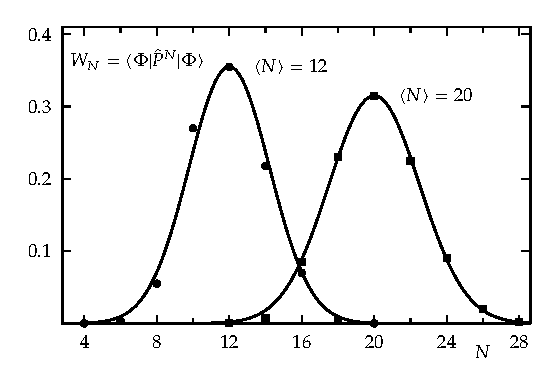
\includegraphics[width=0.6\linewidth]{pictures/11_6}
\par\end{centering}
\centering{}\caption{\label{fig:11_6}稀土区域中实际原子核的BCS基态波函数中具有 $N$ 个粒子、平均数为 $\langle N\rangle={12}$
和 $\langle N\rangle={20}$ 的概率分量。}
\end{figure}

角动量的情况则大不相同。图11.7展示了通过自洽转动模型针对不同 $\left\langle {\widehat{J}}_{x}\right\rangle $
值计算得到的形变良好的原子核 $^{164}\mathrm{{Er}}$ 的内禀波函数中不同角动量的分量 ${W}_{I}$ {[}式（11.150）{]}。现在我们有很强的对称性破缺：
$\left\langle {\Delta{\widehat{\boldsymbol{J}}}^{2}}\right\rangle \simeq{100}$
，这对应于角度上大约 ${10}^{\circ}$ 的展宽，确实是一个相当尖锐的分布。在基态波函数中， $I=0$ 仅由一个相对较小的分量表示。最大值位于
$I\simeq6$ 处。这种意外行为的原因是角动量不是可加量，并且在所考虑的组态空间中，耦合到 $I=6$ 的可能性比耦合到
$I=0$ 的可能性要多得多。由于我们有兴趣以广义直积态的形式考虑尽可能多的关联，我们必须允许存在这样大的赝分量。投影将所有这些分量都设为零。只有在高自旋极限下，分布的最大值才位于
${\widehat{J}}_{x}$ 的平均值处。

\begin{figure}[H]
\begin{centering}
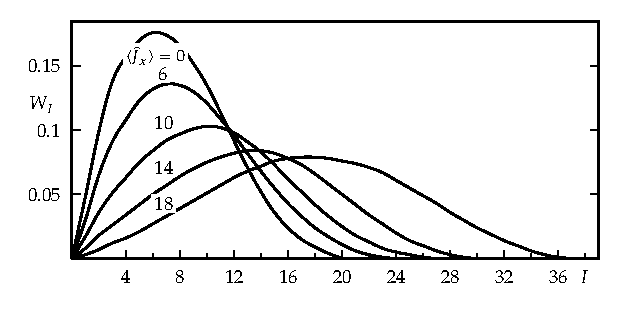
\includegraphics[width=0.62\linewidth]{pictures/11_7}
\par\end{centering}
\centering{}\caption{\label{fig:11_7}对于 $\left\langle {\widehat{J}}_{x}\right\rangle =\sqrt{I\left({I+1}\right)}$
的不同值， $^{164}\mathrm{{Er}}$ 的HFB波函数中具有角动量 $I$ 的概率分量。（源自\cite{IMR79}。）}
\end{figure}

